% Make \texttt safe in PDF strings (prevents hyperref warnings about tokens not allowed in PDF strings)
\ifdefined\pdfstringdefDisableCommands
  \pdfstringdefDisableCommands{\def\texttt#1{#1}}
\fi

\section{Cleaning The Soil Dataset}

\subsection{Handling missing values}

Before any modelling step, missing values were inspected and handled in a controlled way.
The soil table contains both \textit{numeric} variables (e.g., \texttt{SAND}, \texttt{CLAY}, \texttt{REF\_BULK}) and \textit{nominal} (categorical) variables (e.g., \texttt{TEXTURE\_USDA}, \texttt{TEXTURE\_SOTER}), which require different strategies.

\subsubsection{Global inspection and spatial check}

A global missingness score was computed by counting all null cells relative to the total number of cells in the dataset (\textit{missing percentage}).
Rows containing at least one missing value were extracted into a dedicated subset to quantify, for each column, the proportion of missing observations.
This step allows the identification of which soil variables are responsible for most incomplete rows.

To ensure that missingness was not spatially structured (for example concentrated in a specific region), a compact geospatial visualization was produced.
Instead of generating one map per feature, all numeric variables were displayed using a single grid of subplots, providing a global view of their spatial variation while keeping the report concise.
see Annex~\ref{annexe:soil-cleaning-summary} illustrates these spatial patterns and confirms the expected geographic heterogeneity of soil properties across the study area.

\subsubsection{Cross-check of missing patterns for key variables}

A targeted diagnostic was performed on two critical attributes:
\texttt{TEXTURE\_USDA} (categorical soil texture class) and \texttt{REF\_BULK} (reference bulk density).
The goal was to verify whether missing values appear jointly or independently.
The indices of rows with missing soil data were stored, then highlighted in scatter plots as red points aligned at a baseline.
This makes missingness immediately visible as discrete ``gaps'' in the variable signal across the dataset index.
Figure~\ref{fig:soil-missing-scatter} shows that missing values are present but limited, and that the variables do not necessarily become missing in the same rows.

A complementary boxplot analysis was used to summarize the distribution of \texttt{TEXTURE\_USDA} and \texttt{REF\_BULK} and to identify potential outliers.
Histograms were also generated for \texttt{TEXTURE\_USDA} (before and after imputation) to verify that the overall class structure is preserved.
Finally, an ECDF (empirical cumulative distribution function) and a density plot were used for \texttt{REF\_BULK} to better understand its distribution and quartile structure before imputation.

\begin{figure}[H]
    \centering
    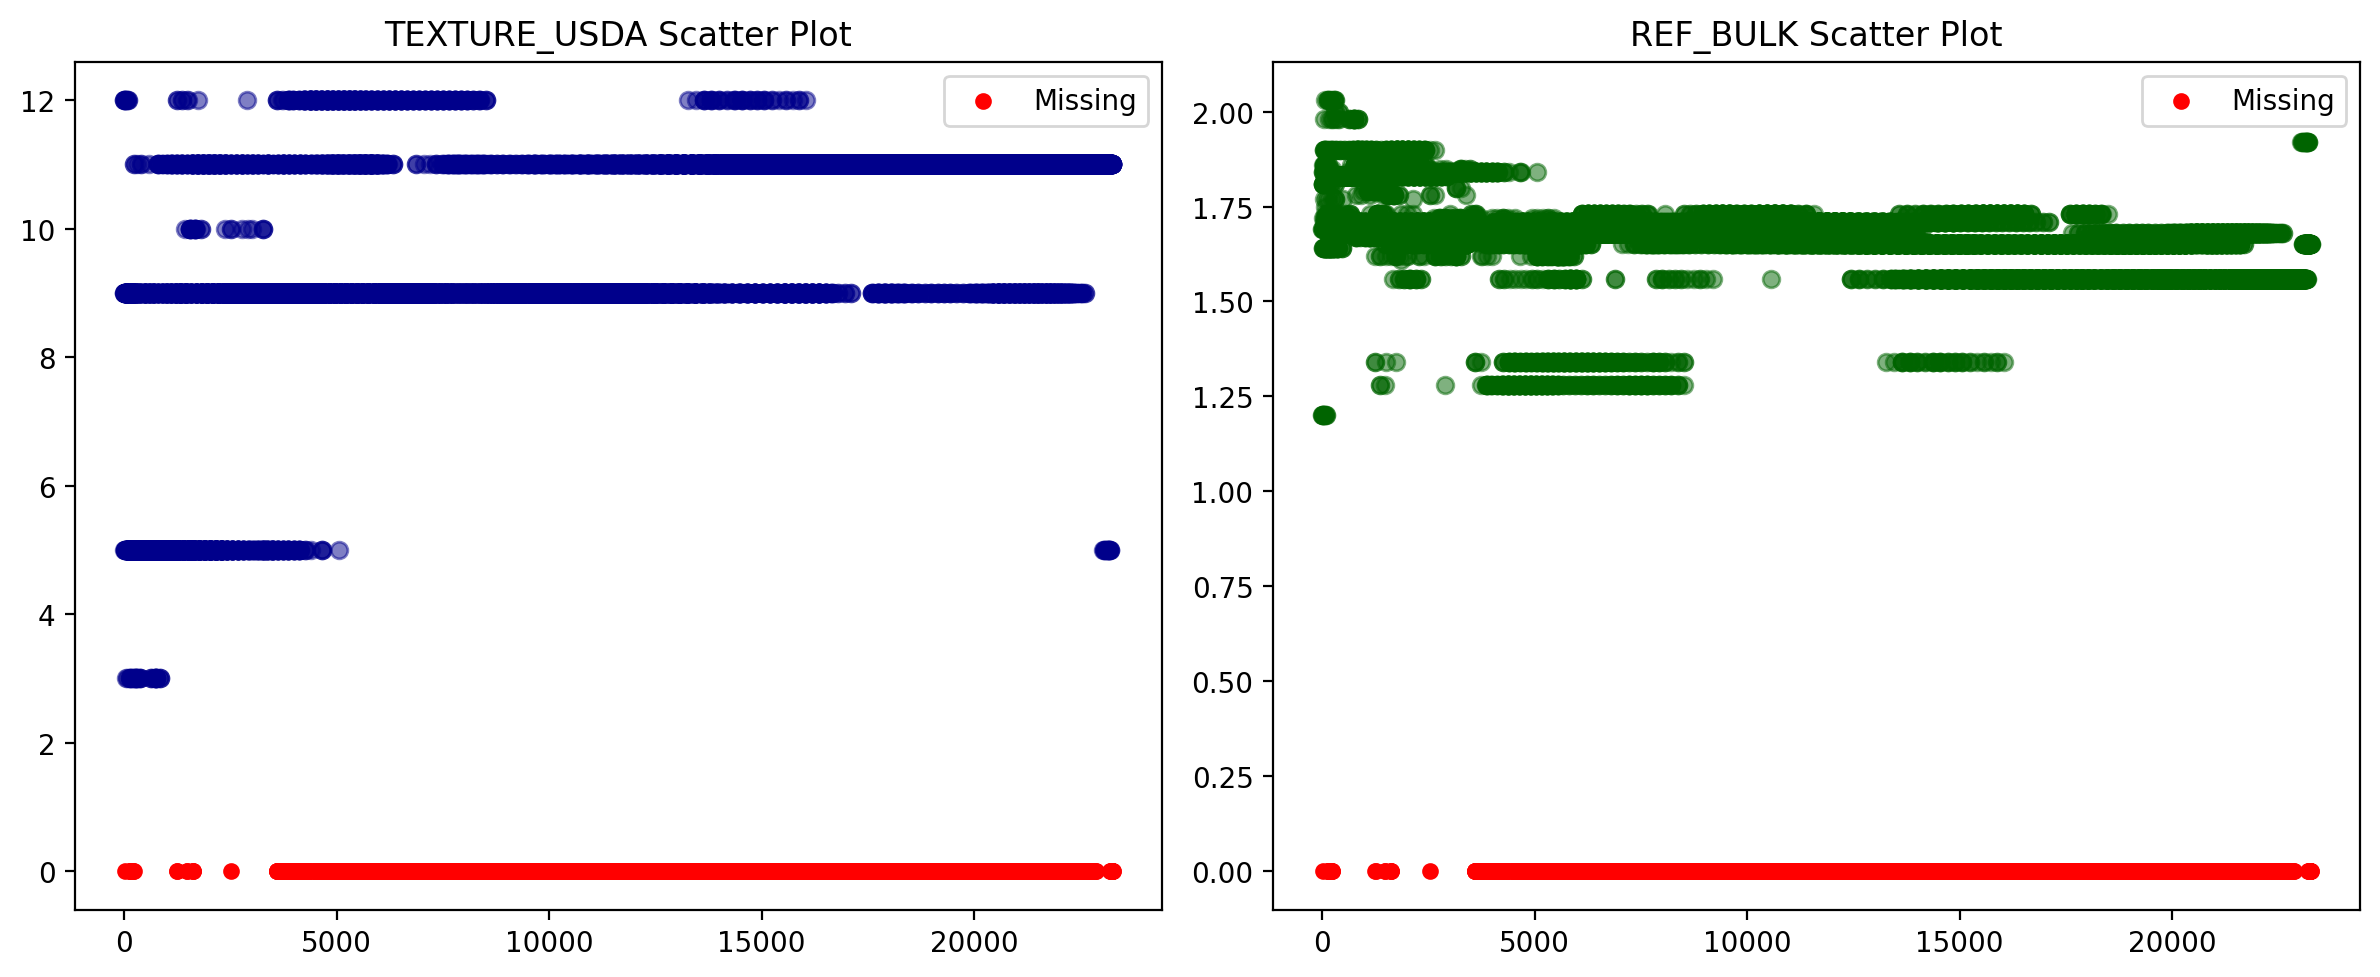
\includegraphics[width=0.5\textwidth]{images/Soil/soil_scatter_texture_refbulk}
    \caption{Scatter plots showing missing values (red markers) for \texttt{TEXTURE\_USDA} and \texttt{REF\_BULK}.}\label{fig:soil-missing-scatter}
\end{figure}

\subsubsection{Imputation of \texttt{REF\_BULK} (numeric)}

For \texttt{REF\_BULK}, missing values were imputed using a simple and robust strategy:
\textbf{median imputation}.
The median is resistant to skewness and extreme values, which is appropriate given the non-Gaussian behaviour observed in several soil variables.
To ensure that the imputation did not distort the variable distribution, kernel density estimates were compared before and after the imputer.
Figures~\ref{fig:soil-refbulk-kde} show that the global density shape remains consistent after filling missing values.

\begin{figure}[H]
    \centering
    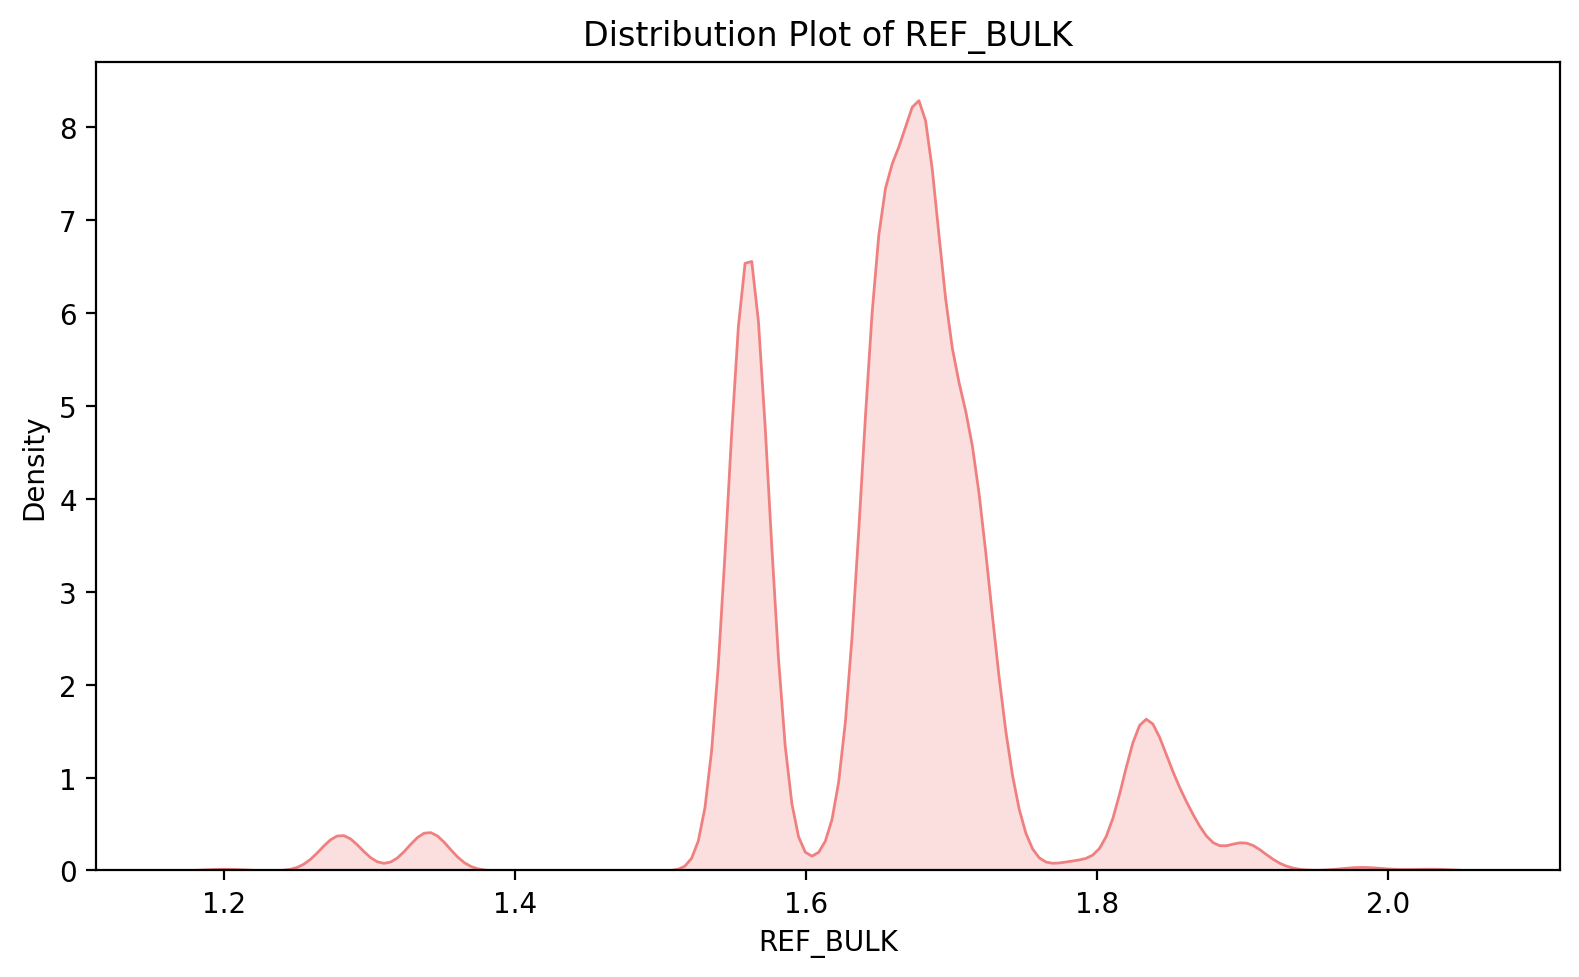
\includegraphics[width=0.35\textwidth]{images/Soil/soil_kde_ref_bulk}
    \hspace{0.05\textwidth}
    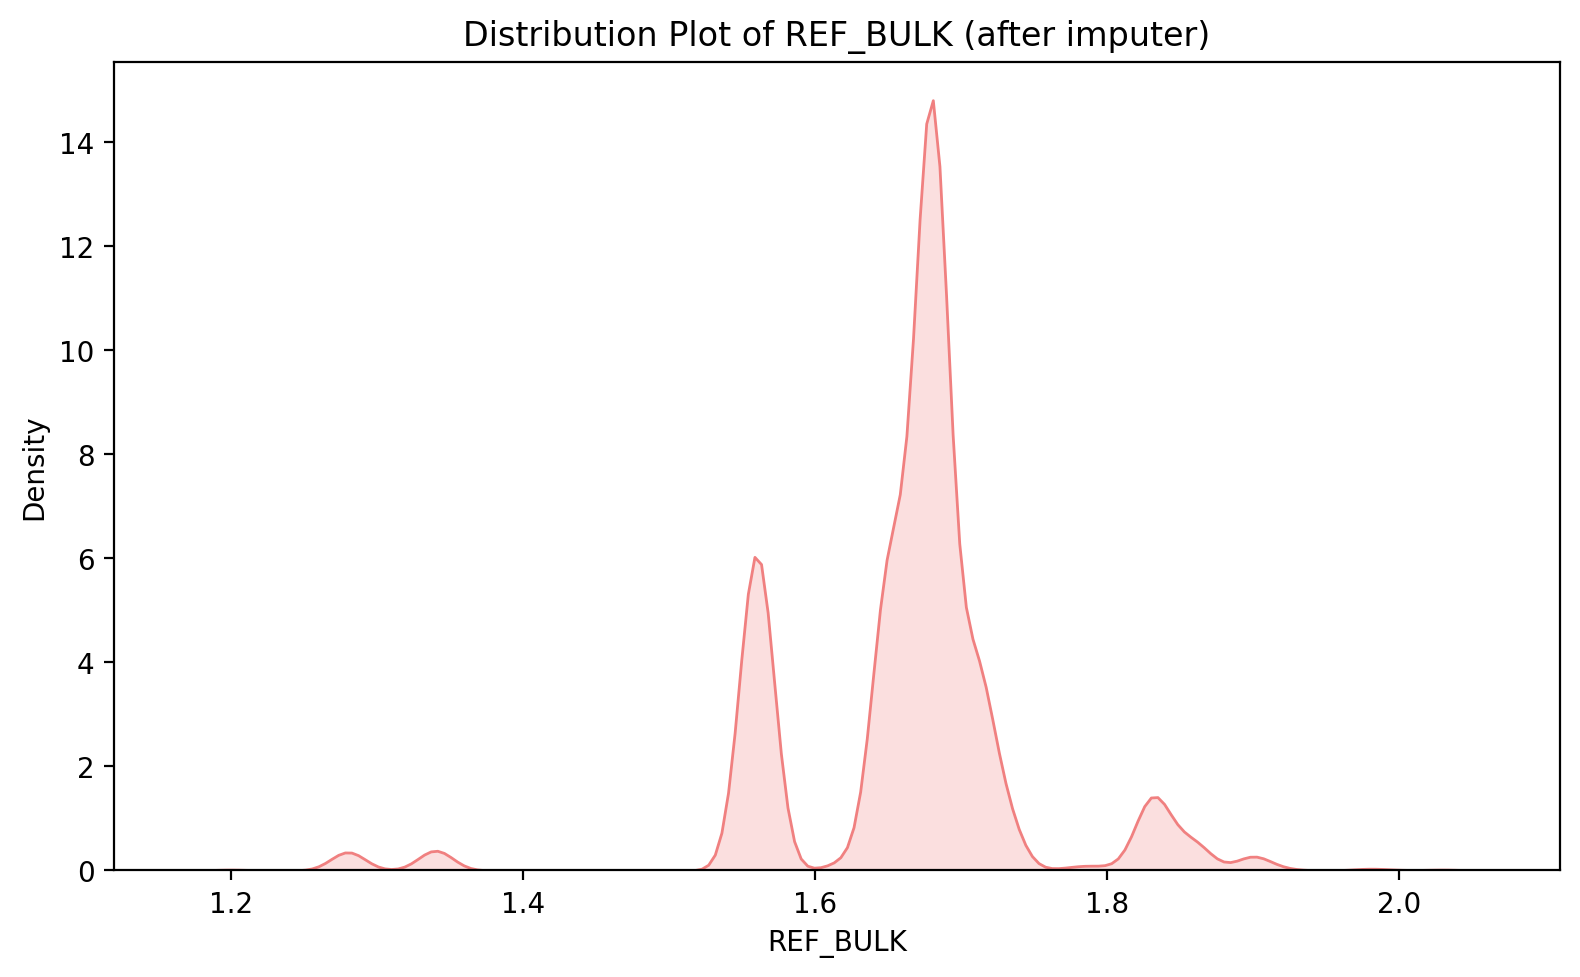
\includegraphics[width=0.35\textwidth]{images/Soil/soil_kde_ref_bulk_after_imputation}
    \caption{Density plot of \texttt{REF\_BULK} before (left) and after (right) median imputation.}\label{fig:soil-refbulk-kde}
\end{figure}

\subsubsection{Imputation of \texttt{TEXTURE\_USDA} (categorical) using composition similarity}

For \texttt{TEXTURE\_USDA}, a direct statistical imputation (mean/median) is not meaningful because the variable is categorical.
Instead, a \textbf{data-driven imputation} was adopted using the numeric texture composition:
\texttt{SAND}, \texttt{SILT}, and \texttt{CLAY}.

Only rows with known \texttt{TEXTURE\_USDA} were used to learn typical texture ``profiles'' per class.
First, the three composition variables were standardized so that Euclidean distances are computed fairly across dimensions.
Then, class centroids were computed as the mean standardized composition for each known USDA class.
For each row with missing \texttt{TEXTURE\_USDA}, its standardized composition was compared to all class centroids, and the closest centroid (minimum Euclidean distance) defined the imputed class.
This approach preserves the physical meaning of USDA texture classes, since the imputation is guided by the sand-silt-clay balance rather than arbitrary label filling.

Finally, the remaining number of missing values in \texttt{TEXTURE\_USDA} was checked to ensure completeness.
The class distribution was also recomputed after imputation, and a histogram was generated to confirm that the imputation did not introduce unrealistic class artefacts.
Figures~\ref{fig:soil-texture-hist} show the distribution before and after imputation.

\begin{figure}[H]
    \centering
    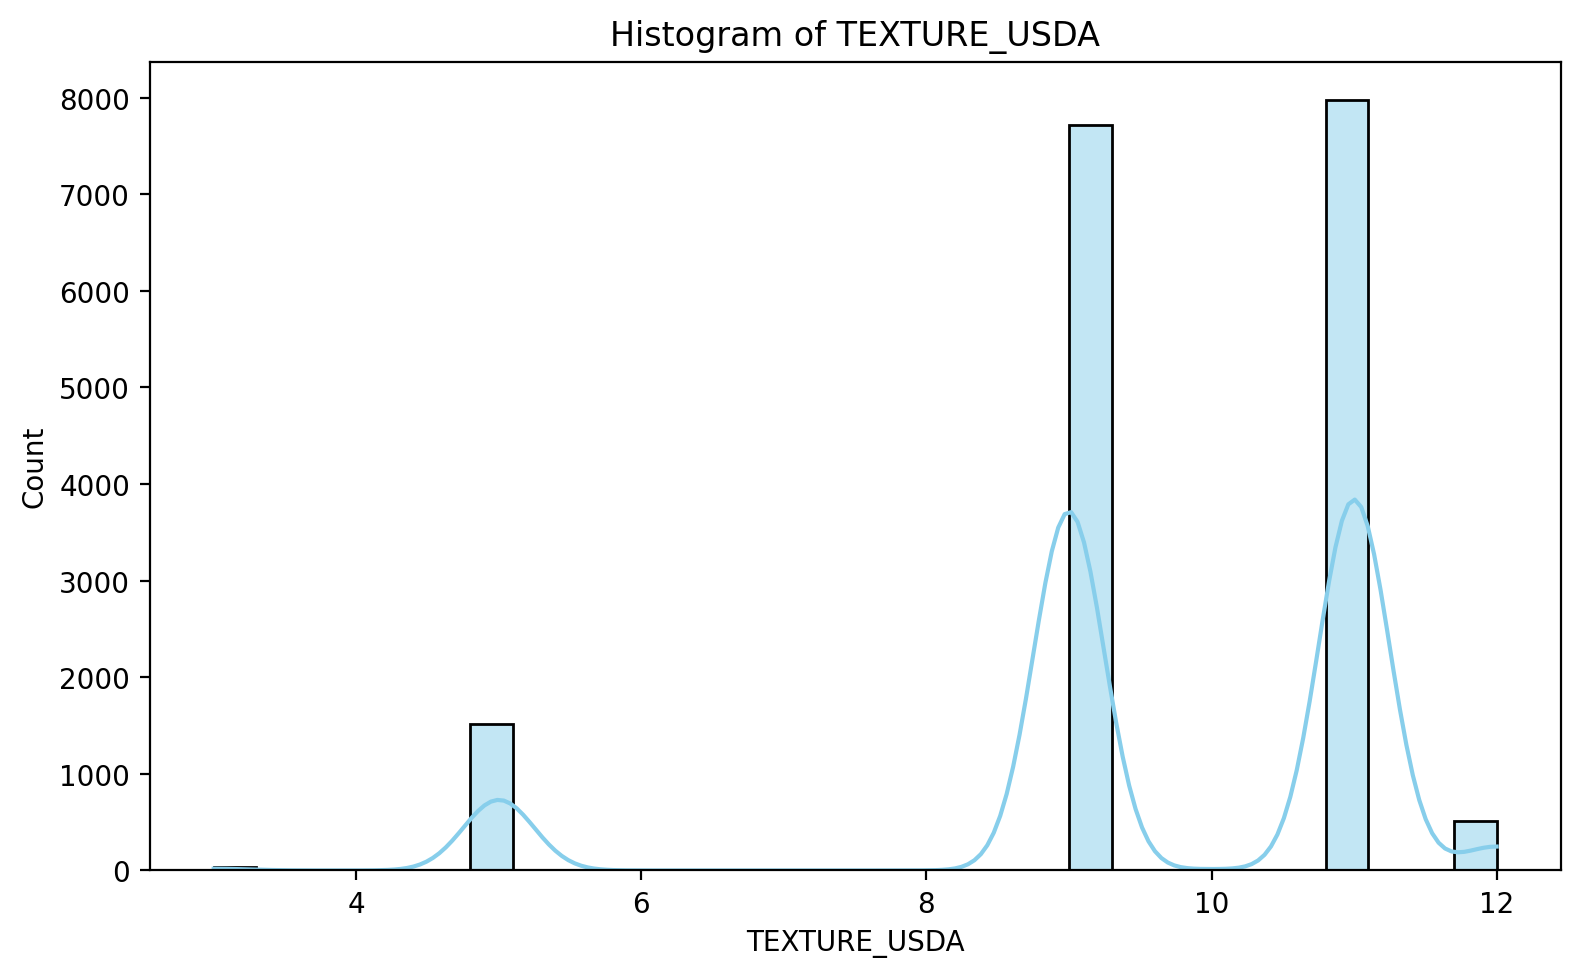
\includegraphics[width=0.35\textwidth]{images/Soil/soil_hist_texture_usda}
    \hspace{0.05\textwidth}
    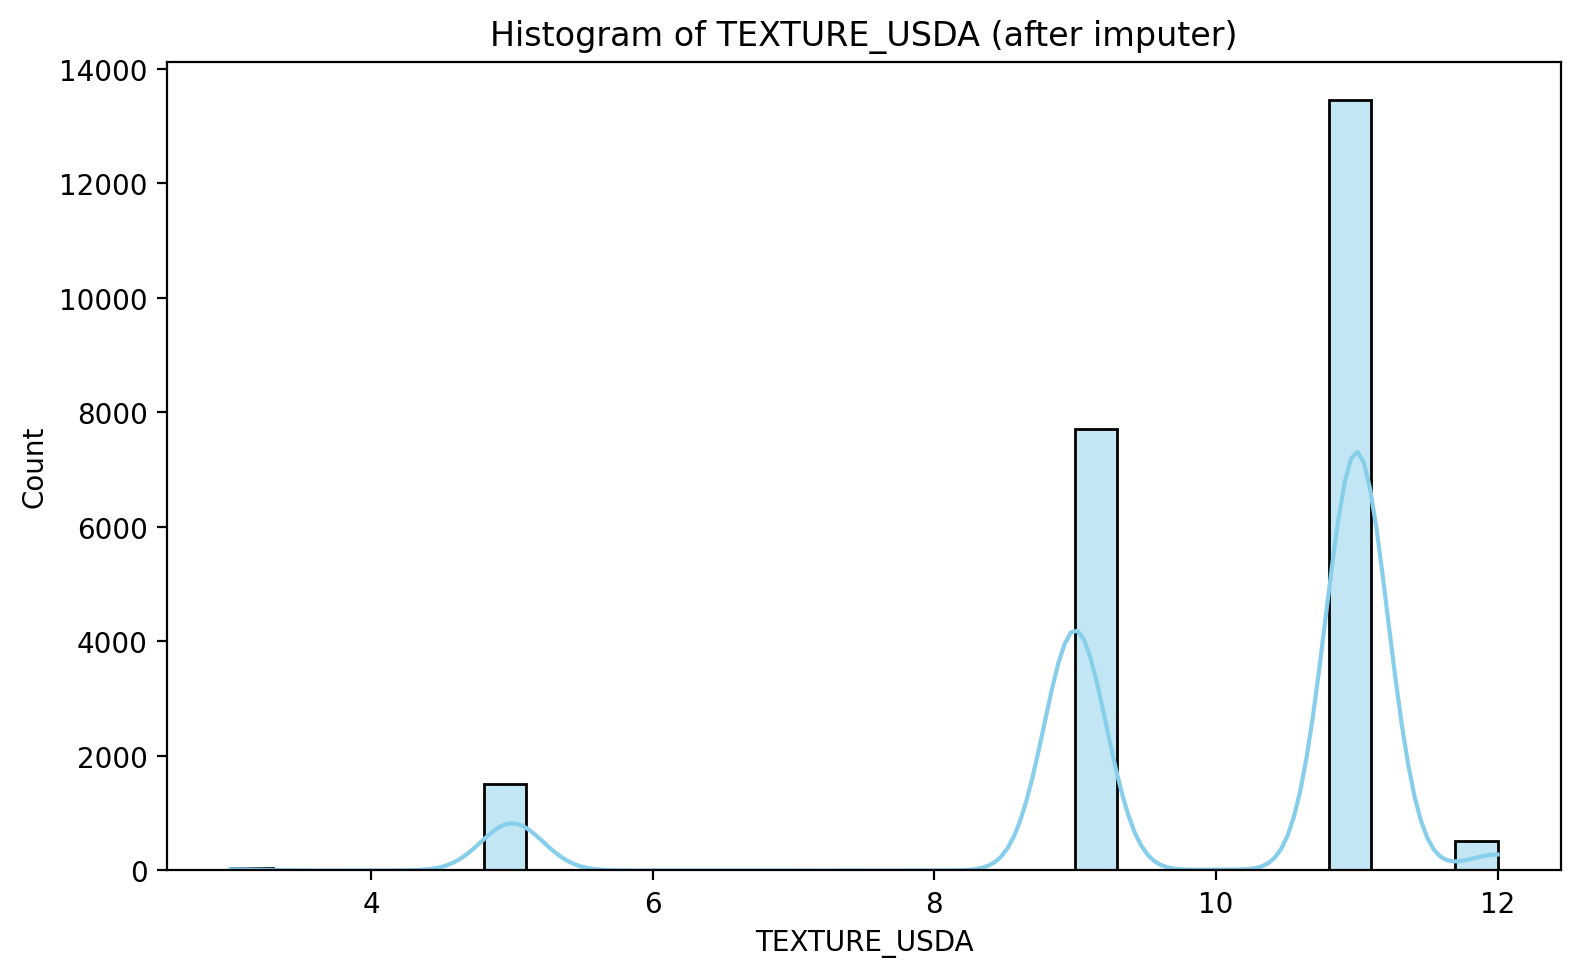
\includegraphics[width=0.35\textwidth]{images/Soil/soil_hist_texture_usda_after_imputer}
    \caption{Histogram of \texttt{TEXTURE\_USDA} before imputation (left, known classes only) and after smart imputation using nearest centroid (right, based on \texttt{SAND}, \texttt{SILT}, \texttt{CLAY}).}\label{fig:soil-texture-hist}
\end{figure}

\subsubsection{Rationale}

This missing-value strategy is intentionally conservative:
median filling for a numeric variable (\texttt{REF\_BULK}) to minimize distribution drift,
and centroid-based imputation for a categorical variable (\texttt{TEXTURE\_USDA}) to preserve soil-texture semantics.
The result is a complete soil feature table that remains consistent with the original spatial and statistical structure of the dataset.


\subsection{Handling Outliers and Invalid Values}\label{subsec:handling_outliers}

\subsubsection{Problem: Negative Values in Soil Properties}

During the exploratory analysis of the soil dataset, a large number of outlier values were identified that are physically impossible. In particular, several soil properties exhibited negative values, including bulk density, soil pH, organic carbon content, electrical conductivity, total nitrogen, C:N ratio, base saturation, aluminum saturation, exchangeable sodium percentage, and gypsum content. Such values are invalid from a pedological perspective, as these variables are strictly non-negative by definition (e.g., pH is bounded within a 0--14 scale, and bulk density must be positive).

A systematic inspection of all numeric soil attributes revealed that exactly \textbf{5,480 records} contained negative values simultaneously across all key soil chemistry variables. This strong co-occurrence strongly suggests that these records correspond to missing data encoded as negative placeholders or to data ingestion errors rather than true soil measurements. Consequently, these records were flagged as invalid outliers requiring correction.

\subsubsection{Detection and Visualization of Invalid Records}

\noindent
\begin{minipage}[t]{0.56\textwidth}
\vspace{0pt}
Initial outlier detection using a generic statistical function (\texttt{detect\_outliers}) reported abnormally high counts of extreme values in several columns, such as approximately 10,961 outliers in gypsum and 9,976 in the C:N ratio. These unexpectedly high numbers suggested a structural issue in the dataset rather than isolated anomalies.

To confirm this hypothesis, each numeric soil variable was explicitly tested for negative values. All critical soil parameters listed above showed the same number of negative entries (5,480), and a cross-check of row indices confirmed that these negative values occurred in the \emph{same set of rows}. These records were therefore classified as globally invalid soil observations.

To assess whether these invalid records were spatially localized or randomly distributed, their geographic distribution was visualized. The soil dataset was converted into a GeoDataFrame using longitude and latitude coordinates, and a spatial scatter map was generated. Valid observations were displayed in light gray, while invalid observations were highlighted in blue (Figure~\ref{fig:invalid_spatial}).
\end{minipage}
\hfill
\begin{minipage}[t]{0.40\textwidth}
\vspace{0pt}
\centering
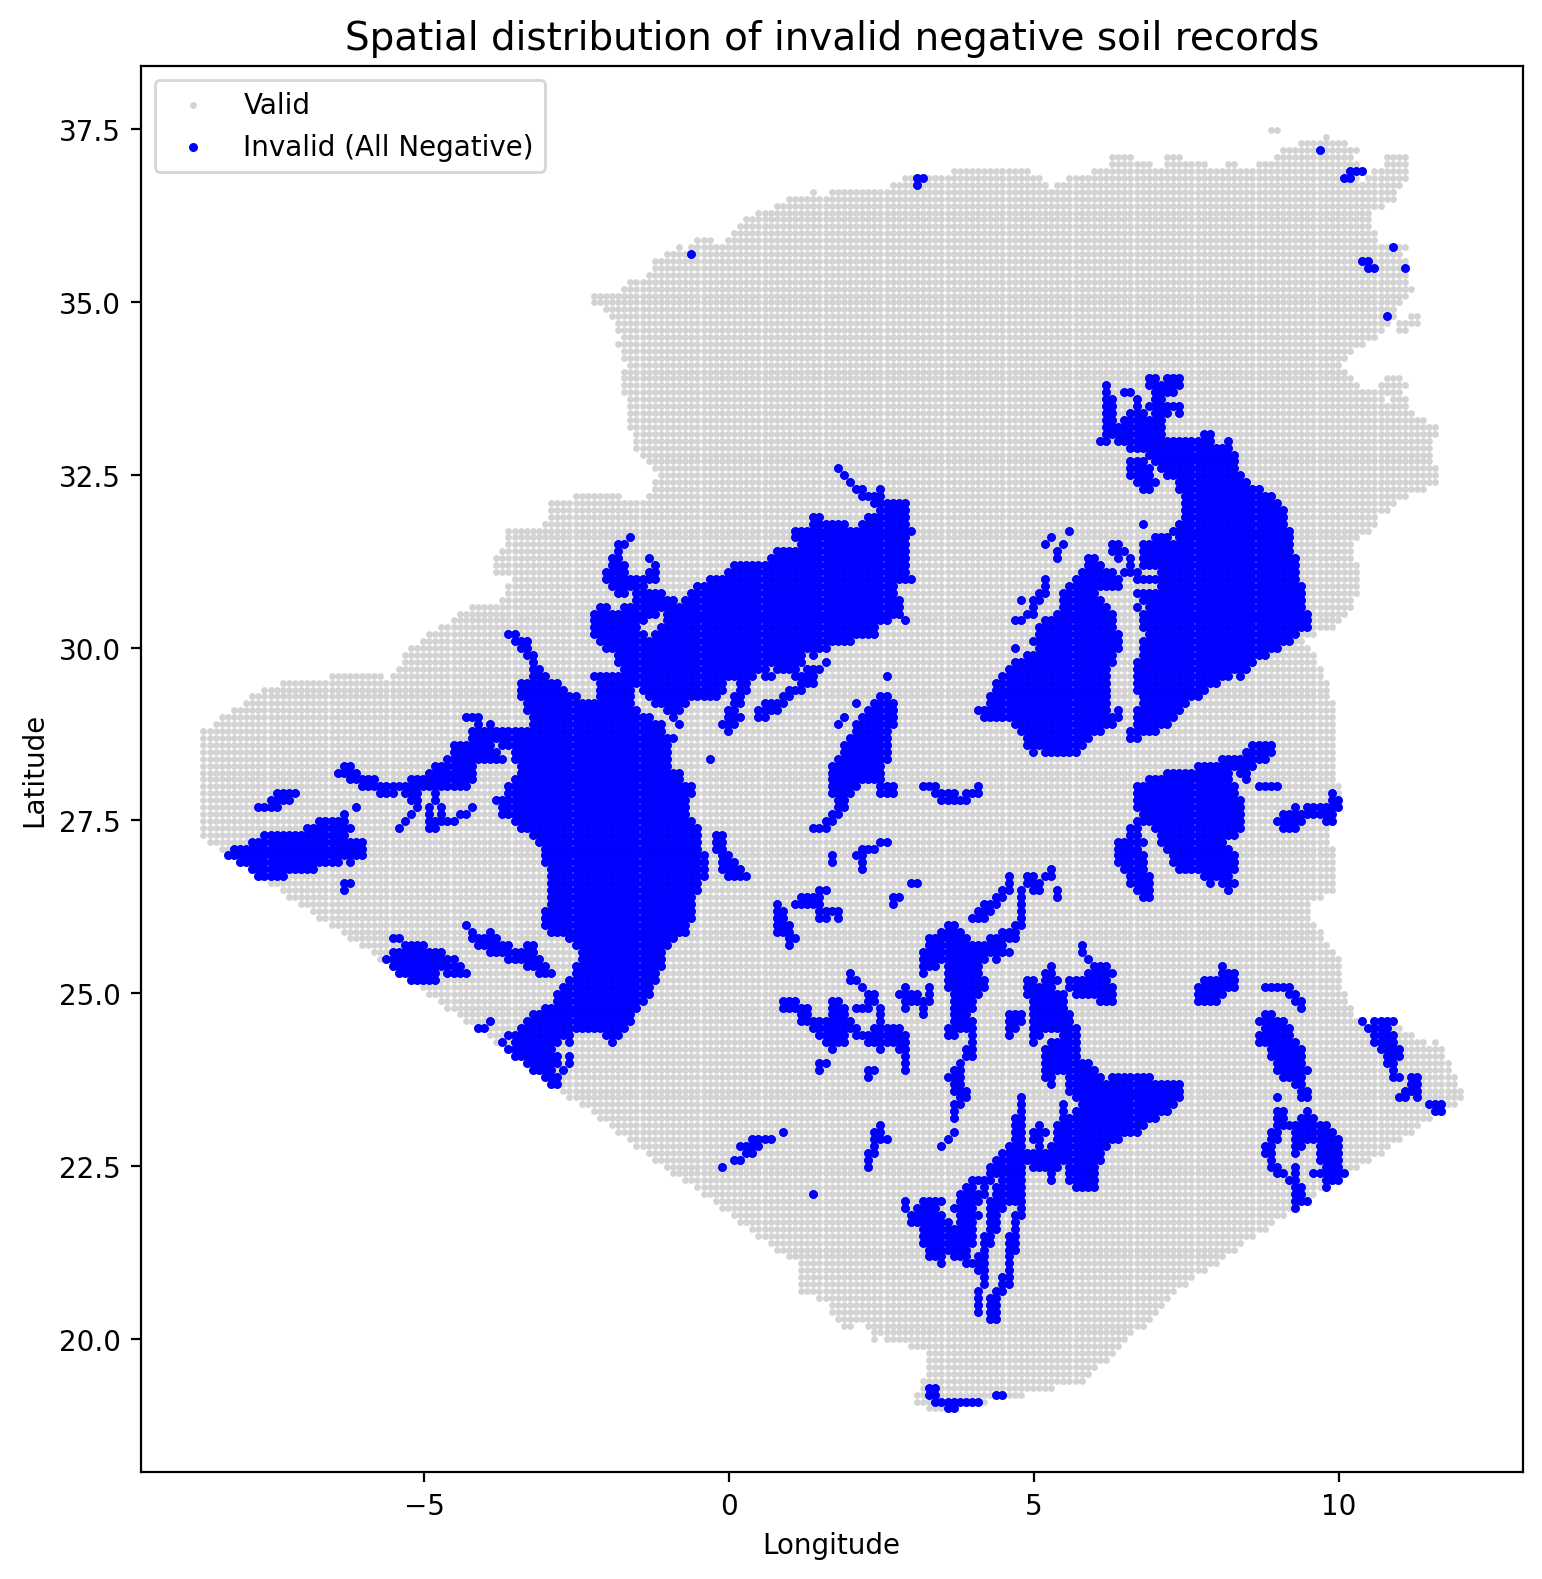
\includegraphics[width=\linewidth]{images/Soil/soil_invalid_negative_spatial_distribution.png}
\captionof{figure}{Spatial distribution of invalid soil records with negative values. Valid points are shown in light gray, while invalid points (all key soil properties negative) are highlighted in blue.}
\label{fig:invalid_spatial}
\end{minipage}

\subsubsection{Solution: Nearest-Neighbor Imputation of Invalid Values}

Rather than discarding more than five thousand soil records---which would have introduced spatial gaps and potential bias---a nearest-neighbor imputation strategy was adopted. The objective was to replace invalid values with representative estimates derived from geographically nearby valid observations. For each invalid record, the median value of its neighboring valid points was used for imputation. The median was preferred over the mean due to its robustness to local variability and residual outliers, while still preserving local soil characteristics.

\subsubsection{Imputation Procedure}

The imputation workflow was implemented as follows:

\begin{enumerate}
    \item \textbf{Identification of Invalid Records}: A boolean mask (\texttt{is\_invalid}) was created to identify rows where all targeted physical soil attributes were negative.
    \item \textbf{Preparation of Spatial Data}: All coordinates were ensured to be expressed in WGS84 latitude/longitude and converted to radians, as required for great-circle distance calculations.
    \item \textbf{Construction of a BallTree}: A BallTree data structure was built using only valid soil records, with the haversine distance metric see Annex~\ref{annexe:soil-cleaning-summary}. This structure enables efficient spatial nearest-neighbor searches.
    \item \textbf{Neighbor Querying}: For each invalid record, the 8 nearest valid neighbors within a 100~km radius were queried. If no valid neighbors were found within this radius, the 8 nearest neighbors were retrieved regardless of distance.
    \item \textbf{Median-Based Imputation}: For each numeric soil attribute, the median of the neighboring valid values was computed and used to replace the invalid negative value. As all imputed attributes were numeric, no categorical imputation was required.
    \item \textbf{Dataset Update}: The DataFrame was updated with the imputed values, and an audit check confirmed that no records remained with all-negative soil attributes.
\end{enumerate}

\subsubsection{Post-Imputation Validation}
After imputation, \textbf{ all 5,480 previously invalid records were corrected}. We verified that no record now has all negative values in the key soil columns (the count of fully-invalid rows dropped to 0). We also generated a new spatial plot: the blue points indicating invalid records have disappeared, confirming that our imputation filled in plausible values for those locations. The dataset's overall quality improved, as every soil property value is now within a realistic range.
In summary, we detected a large batch of outlier records characterized by impossible negative soil property values. By leveraging spatial nearest-neighbor imputation (with a BallTree for efficient lookup), we replaced those erroneous values with median values from nearby valid data points. This method preserved the spatial trends and continuity of the soil properties while eliminating clearly invalid entries, resulting in a cleaner and more reliable dataset for downstream analysis or modeling.

\begin{figure}[H]
    \centering
    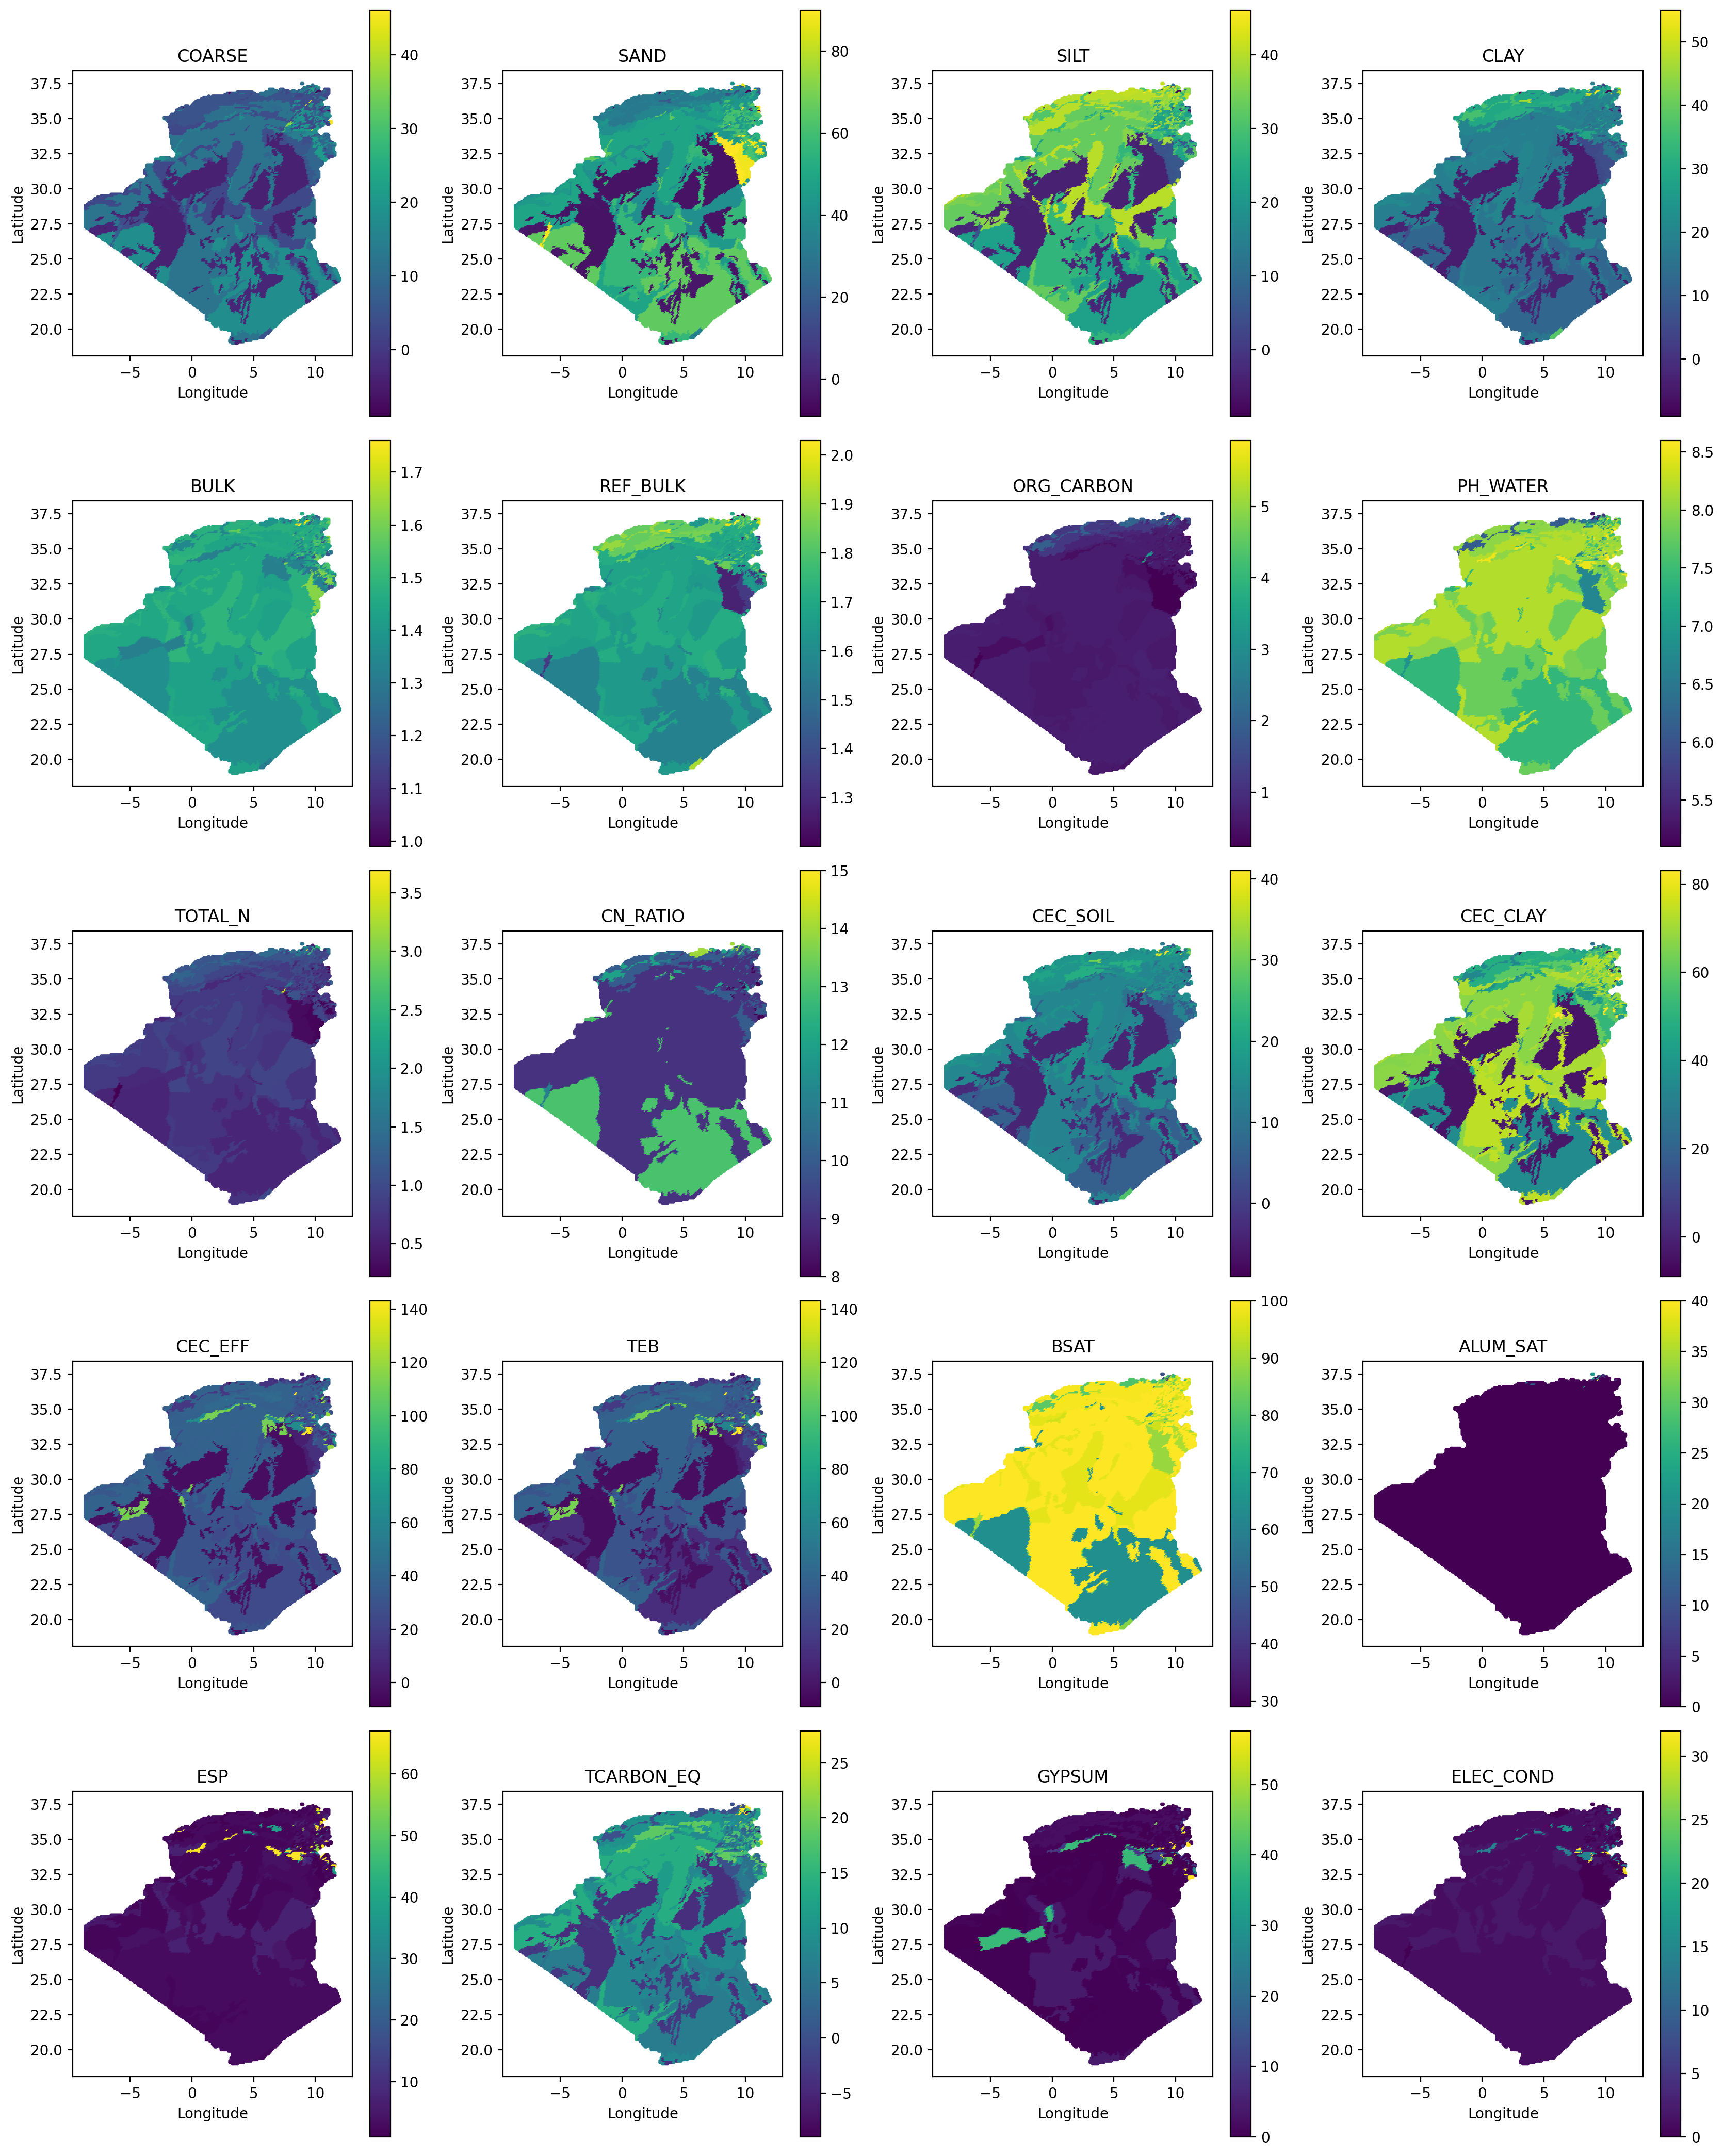
\includegraphics[width=0.65\textwidth]{images/Soil/soil_maps_numeric_variation_after_invalid_imputation}
    \caption{Histograms of soil attributes after nearest-neighbor imputation, showing consistent and physically plausible distributions.}\label{fig:soil_imputation_validation}
\end{figure}
The resulting soil property distributions after imputation are shown in Annex~\ref{annexe:soil-cleaning-summary}, confirming that all variables now exhibit realistic ranges and shapes without negative values.
\subsubsection*{Detected Statistical Outliers}

Using an interquartile-range (IQR)-based detector, the following number of outliers were identified after imputation:

\begin{table}[H]
\centering
\begin{tabular}{l r l r}
\toprule
\textbf{Variable} & \textbf{Outliers} & \textbf{Variable} & \textbf{Outliers} \\
\midrule
COARSE        & 28   & BSAT         & 11   \\
SAND          & 12   & ALUM\_SAT    & 28   \\
SILT          & 0    & ESP          & 4095 \\
CLAY          & 53   & TCARBON\_EQ  & 0    \\
BULK          & 341  & GYPSUM       & 1182 \\
REF\_BULK     & 969  & ELEC\_COND   & 5973 \\
ORG\_CARBON   & 2897 & CEC\_SOIL    & 53   \\
PH\_WATER     & 272  & CEC\_CLAY    & 0    \\
TOTAL\_N      & 190  & CEC\_EFF     & 506  \\
CN\_RATIO     & 1    & TEB          & 506  \\
\bottomrule
\end{tabular}
\caption{Count of statistical outliers detected using the IQR-based method after imputation.}
\label{tab:outlier_counts}
\end{table}


The high outlier counts observed in salinity- and chemistry-related variables (ESP, ELEC\_COND, GYPSUM, ORG\_CARBON) are consistent with arid and semi-arid soil environments, where strong spatial gradients and extreme values are common.

\subsubsection*{Case Focus: REF\_BULK (Reference Bulk Density)}

REF\_BULK represents the expected soil bulk density (g/cm\textsuperscript{3}) derived from pedotransfer functions. Typical mineral soils range between 1.2 and 1.9 g/cm\textsuperscript{3}. Values exceeding 2.0 often indicate compaction, erosion, or crusted soils, while very low values suggest organic-rich or loose substrates. REF\_BULK is a key indicator of soil structure degradation, which can indirectly increase fire susceptibility by limiting infiltration and inducing vegetation stress\cite{nrcs_bulk_density}.

The Quantiles plot of REF\_BULK after imputation shows a near-linear central trend with mild tail deviations, confirming that extreme values are limited and physically interpretable rather than erroneous.

\subsubsection*{Distributional Analysis by Variable Groups}

\paragraph{Texture and Particle-Size Variables}
COARSE, SAND, SILT, and CLAY exhibit multimodal distributions caused by mixed soil texture classes. None follow a normal distribution due to compositional constraints (percentages summing to 100). These variables are better handled through scaling or compositional transformations rather than outlier removal.

\paragraph{Density and Base Properties}
BULK and REF\_BULK show near-normal distributions, whereas PH\_WATER is clearly bimodal, reflecting acidic and alkaline soil regimes. PH\_WATER is therefore not amenable to normalization via standard transformations and is better treated using stratified or non-parametric approaches.

\paragraph{Organic Matter and Nutrients}
TOTAL\_N approximates normality. ORG\_CARBON, CN\_RATIO, and TCARBON\_EQ are strongly skewed and multimodal, reflecting varying organic and inorganic carbon pools across ecosystems.

\paragraph{Cation Exchange and Fertility Indicators}
CEC-related variables and TEB show positive skewness and multi-peaked structures, while BSAT is bounded between 0 and 100, resulting in truncated distributions.

\paragraph{Salinity and Saturation Indicators}
ALUM\_SAT, ESP, GYPSUM, and ELEC\_COND are heavily right-skewed with extreme upper tails. These extremes correspond to saline or sodic soils and are ecologically meaningful rather than erroneous.

\subsubsection*{Methodological Decision}

Importantly, no additional outliers were removed at this stage. Since the detected values are physically plausible and reflect genuine soil variability, removing them could bias the dataset and weaken spatial generalization. Instead, all numeric variables will be handled at later stages using normalization or robust scaling techniques appropriate for machine learning, ensuring model stability without altering the underlying data distribution\cite{wilson2021mlsoil}.

\subsection{Initiation to Feature Engineering: Identification of Redundant Variables}

Feature engineering begins with a careful examination of variable dependencies in order to reduce redundancy, prevent multicollinearity, and preserve only informative predictors. In this study, several soil attributes were identified as deterministic or quasi-deterministic transformations of other variables. These variables were therefore evaluated for potential removal prior to normalization and modeling.

\subsubsection{Redundancy in Soil Texture Variables}

The dataset includes two categorical soil texture indicators:
\begin{itemize}
    \item \texttt{TEXTURE\_USDA}, with unique values \{3, 5, 9, 10, 11, 12\}
    \item \texttt{TEXTURE\_SOTER}, with unique values \{\texttt{M}, \texttt{C}, \texttt{F}, \texttt{-}\}
\end{itemize}

Parallel coordinates plots (Figure~\ref{fig:texture_parallel}) were used to analyze the relationship between these texture classes and the particle-size fractions \texttt{SAND}, \texttt{SILT}, and \texttt{CLAY}.  
When grouped by \texttt{TEXTURE\_USDA}, the trajectories corresponding to each class are clearly separated and internally consistent: each USDA texture category maps to a unique combination of sand, silt, and clay proportions. This confirms that \texttt{TEXTURE\_USDA} is fully determined by these three quantitative variables, as defined by the USDA soil texture triangle.

A similar pattern is observed for \texttt{TEXTURE\_SOTER}. Coarse soils (\texttt{C}) exhibit high sand and low clay contents, fine soils (\texttt{F}) show the opposite behavior, and medium soils (\texttt{M}) occupy intermediate ranges. These groupings align directly with the particle-size composition, indicating that \texttt{TEXTURE\_SOTER} is likewise a categorical encoding derived from \texttt{SAND}, \texttt{SILT}, and \texttt{CLAY}.

Because both texture variables are deterministic functions of the same base fractions, they do not contribute additional independent information. Retaining them would introduce redundancy and multicollinearity. Consequently, both \texttt{TEXTURE\_USDA} and \texttt{TEXTURE\_SOTER} were removed from the feature set.

\begin{figure}[H]
\centering
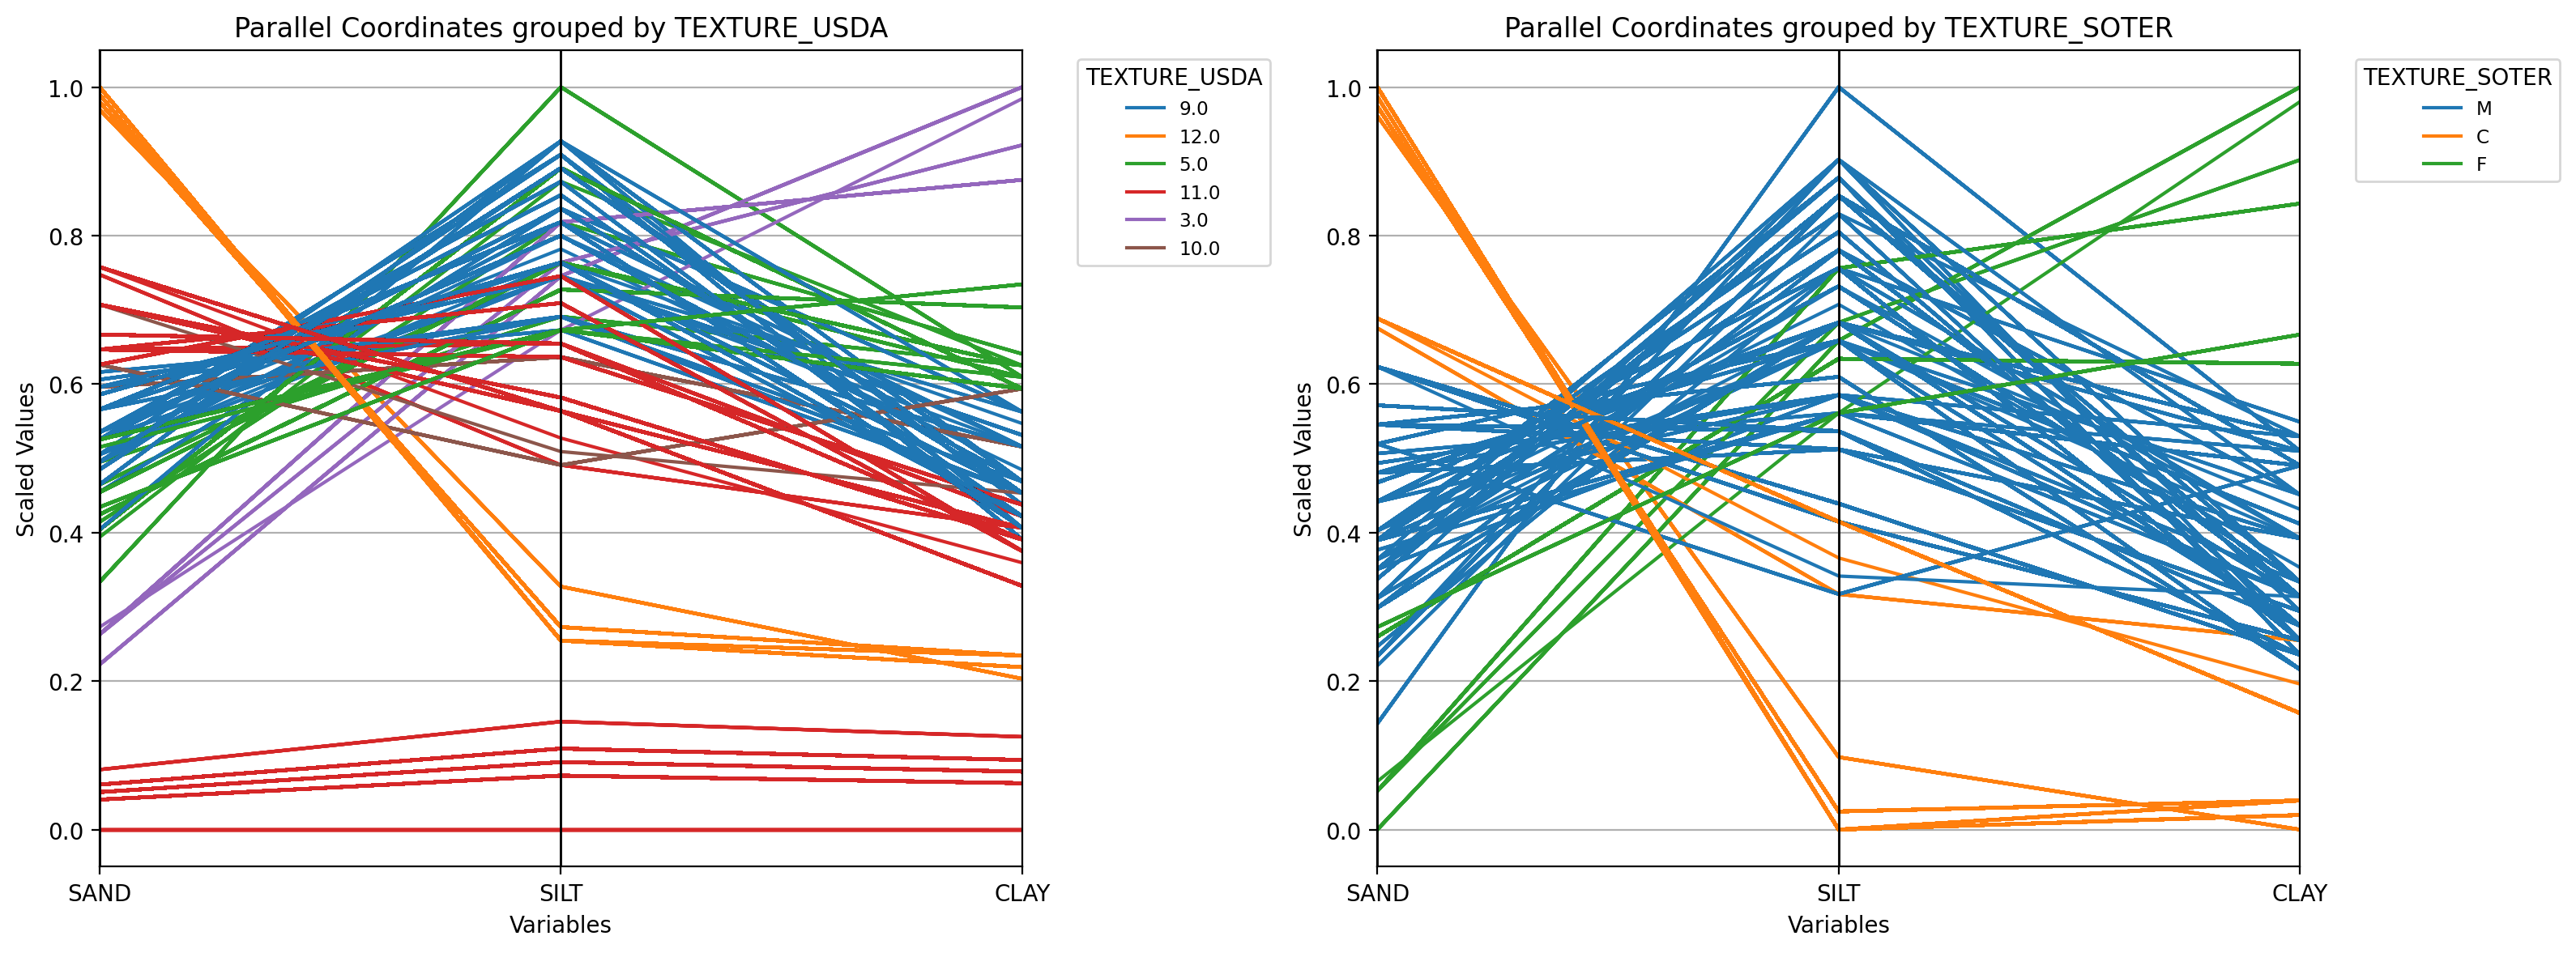
\includegraphics[width=0.55\textwidth]{images/Soil/soil_parallel_coordinates_texture.png}
\caption{Parallel coordinates of particle-size fractions grouped by \texttt{TEXTURE\_USDA} (left) and \texttt{TEXTURE\_SOTER} (right), showing that both texture classes are deterministic encodings of sand, silt, and clay composition.}\label{fig:texture_parallel}
\end{figure}

\subsubsection{Redundancy of the C/N Ratio}

The carbon-to-nitrogen ratio (\texttt{CN\_RATIO}) is defined in the FAO Harmonized World Soil Database as:
\[
\text{CN\_RATIO} = \frac{\text{ORG\_CARBON}}{\text{TOTAL\_N}}
\]

To verify this relationship empirically, the provided \texttt{CN\_RATIO} values were compared with a recomputed ratio obtained directly from \texttt{ORG\_CARBON} divided by \texttt{TOTAL\_N}. The scatter and Q-Q plots (Figure~\ref{fig:cn_ratio}) reveal a near one-to-one correspondence. The Pearson correlation coefficient reaches 0.92 ($p<0.001$), and the Spearman rank correlation is 0.79 ($p<0.001$), confirming a strong deterministic dependency.

Minor deviations from the identity line are attributable to rounding effects and numerical precision in the original dataset. Since \texttt{CN\_RATIO} is a direct transformation of two already available variables, it does not represent an independent soil property. To avoid redundancy, \texttt{CN\_RATIO} was therefore removed, while \texttt{ORG\_CARBON} and \texttt{TOTAL\_N} were retained.

\begin{figure}[H]
\centering
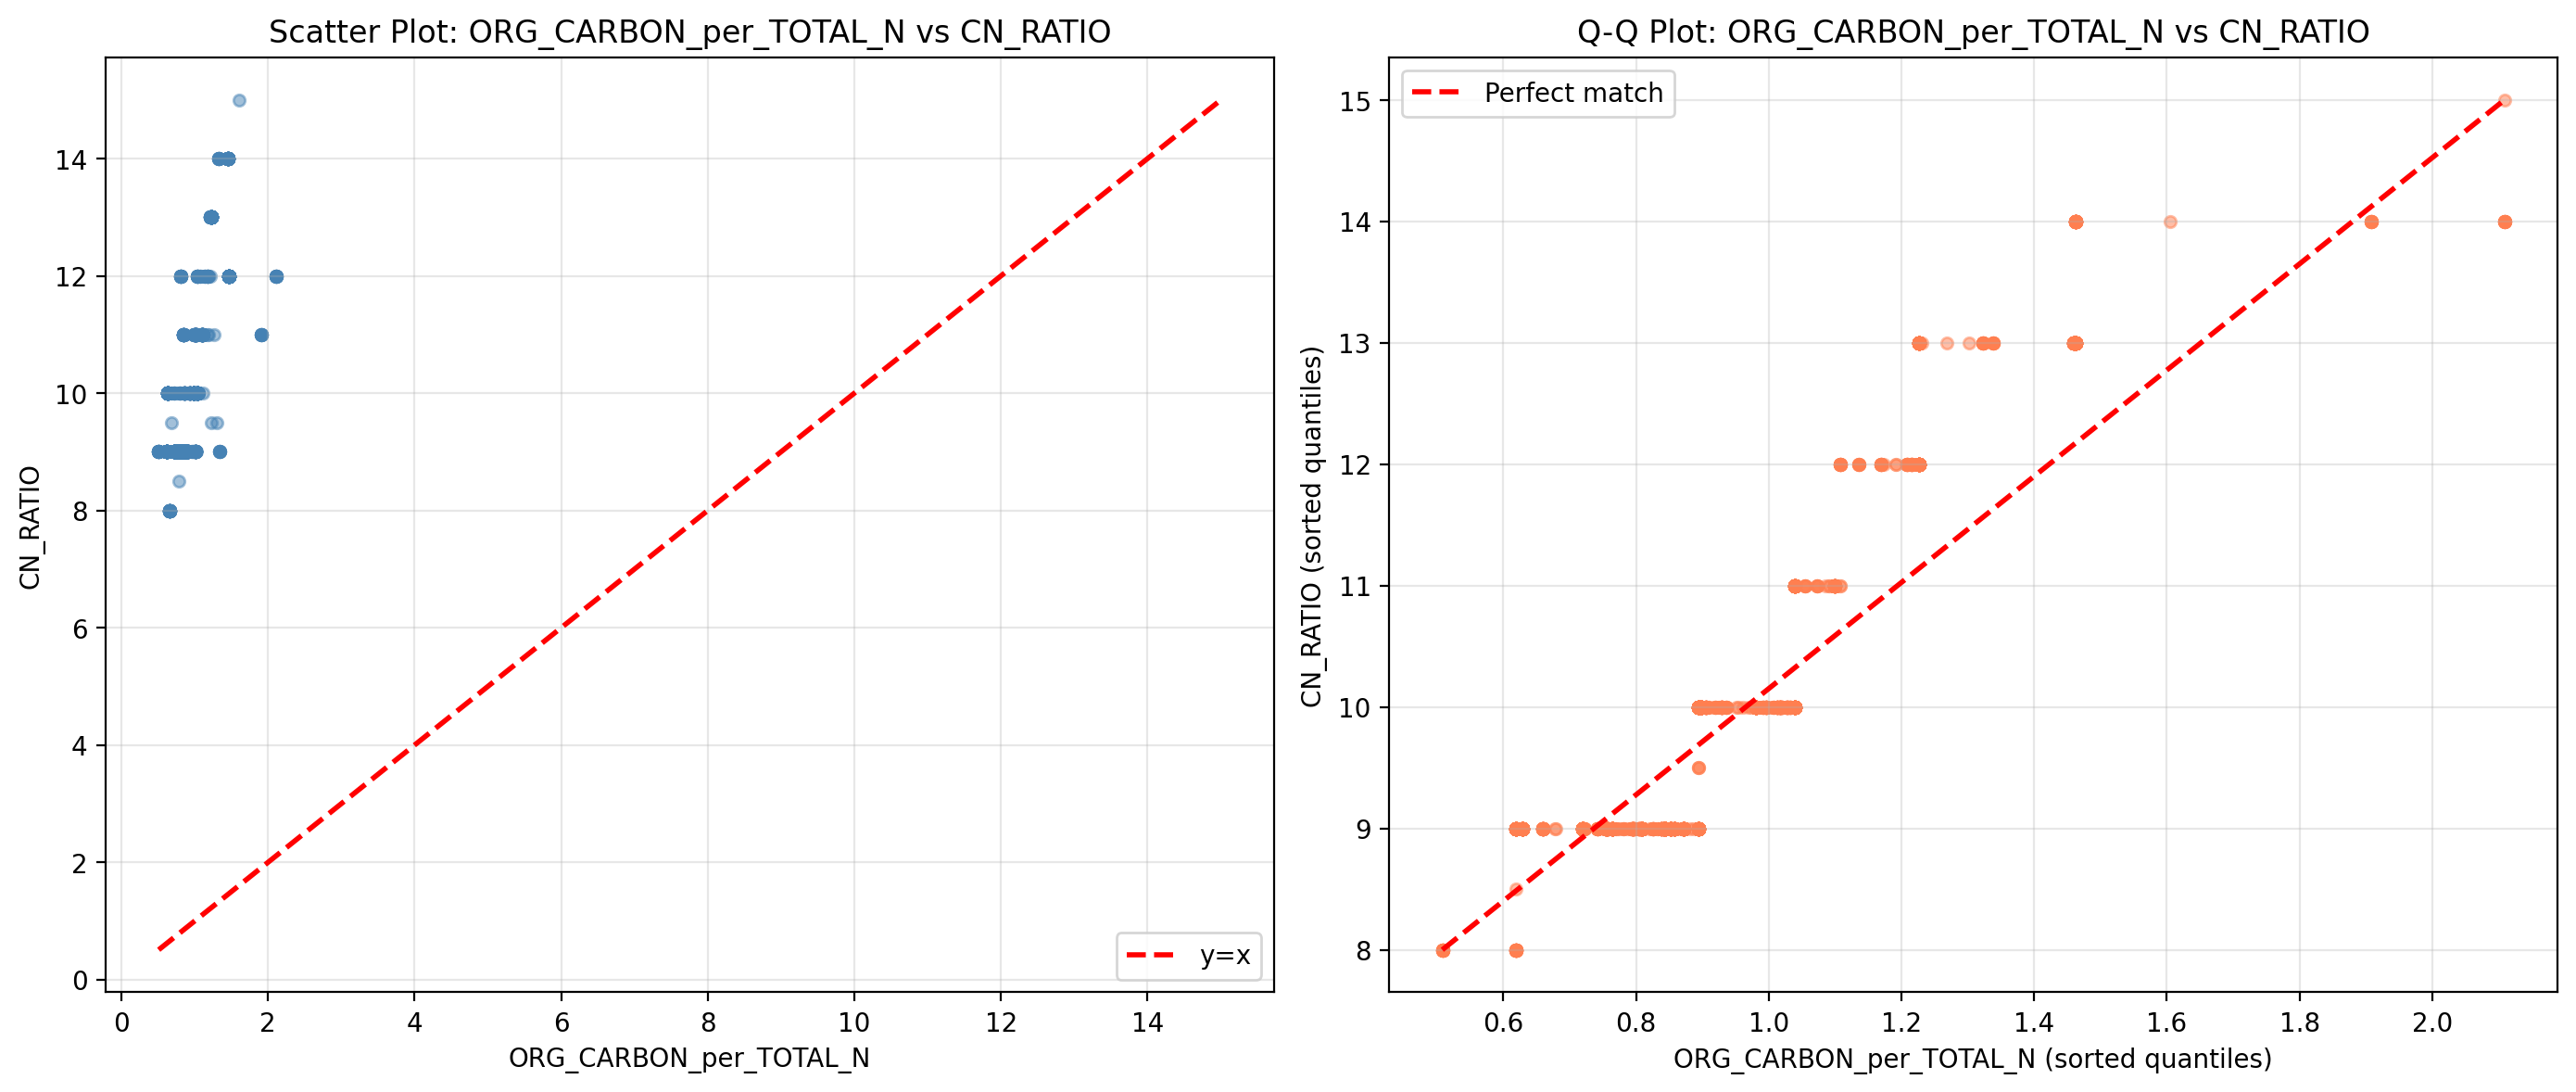
\includegraphics[width=0.55\textwidth]{images/Soil/soil_ORG_CARBON_per_TOTAL_N_vs_CN_RATIO_scatter_qq.png}
\caption{Scatter and Q-Q plots comparing \texttt{CN\_RATIO} to the recomputed ratio \texttt{ORG\_CARBON / TOTAL\_N}, confirming a near-deterministic relationship.}\label{fig:cn_ratio}
\end{figure}

\subsubsection{Relationship Between \texttt{CEC\_SOIL} and \texttt{CEC\_CLAY}}

The Cation Exchange Capacity of clay (\texttt{CEC\_CLAY}) is theoretically approximated as:
\[
\text{CEC}_{\text{clay}} = \frac{\text{CEC}_{\text{soil}}}{\text{Clay fraction}}
\]
as described in pedological literature and FAO documentation.

However, empirical evaluation shows that this theoretical approximation does not hold strictly in practice. The computed ratio \texttt{CEC\_SOIL\_per\_CLAY} exhibits only a weak-to-moderate relationship with the observed \texttt{CEC\_CLAY} (Pearson $r=-0.37$, Spearman $\rho=-0.15$, both $p<0.001$). The scatter and Q--Q plots (Figure~\ref{fig:cec_clay}) show substantial dispersion around the 1:1 line.

This variability reflects the influence of additional factors such as organic matter, silt content, and oxide coatings, which also contribute to soil cation exchange capacity. Therefore, despite their conceptual linkage, \texttt{CEC\_SOIL} and \texttt{CEC\_CLAY} are not redundant. Both variables were retained as complementary indicators of soil chemical behavior.

\begin{figure}[H]
\centering
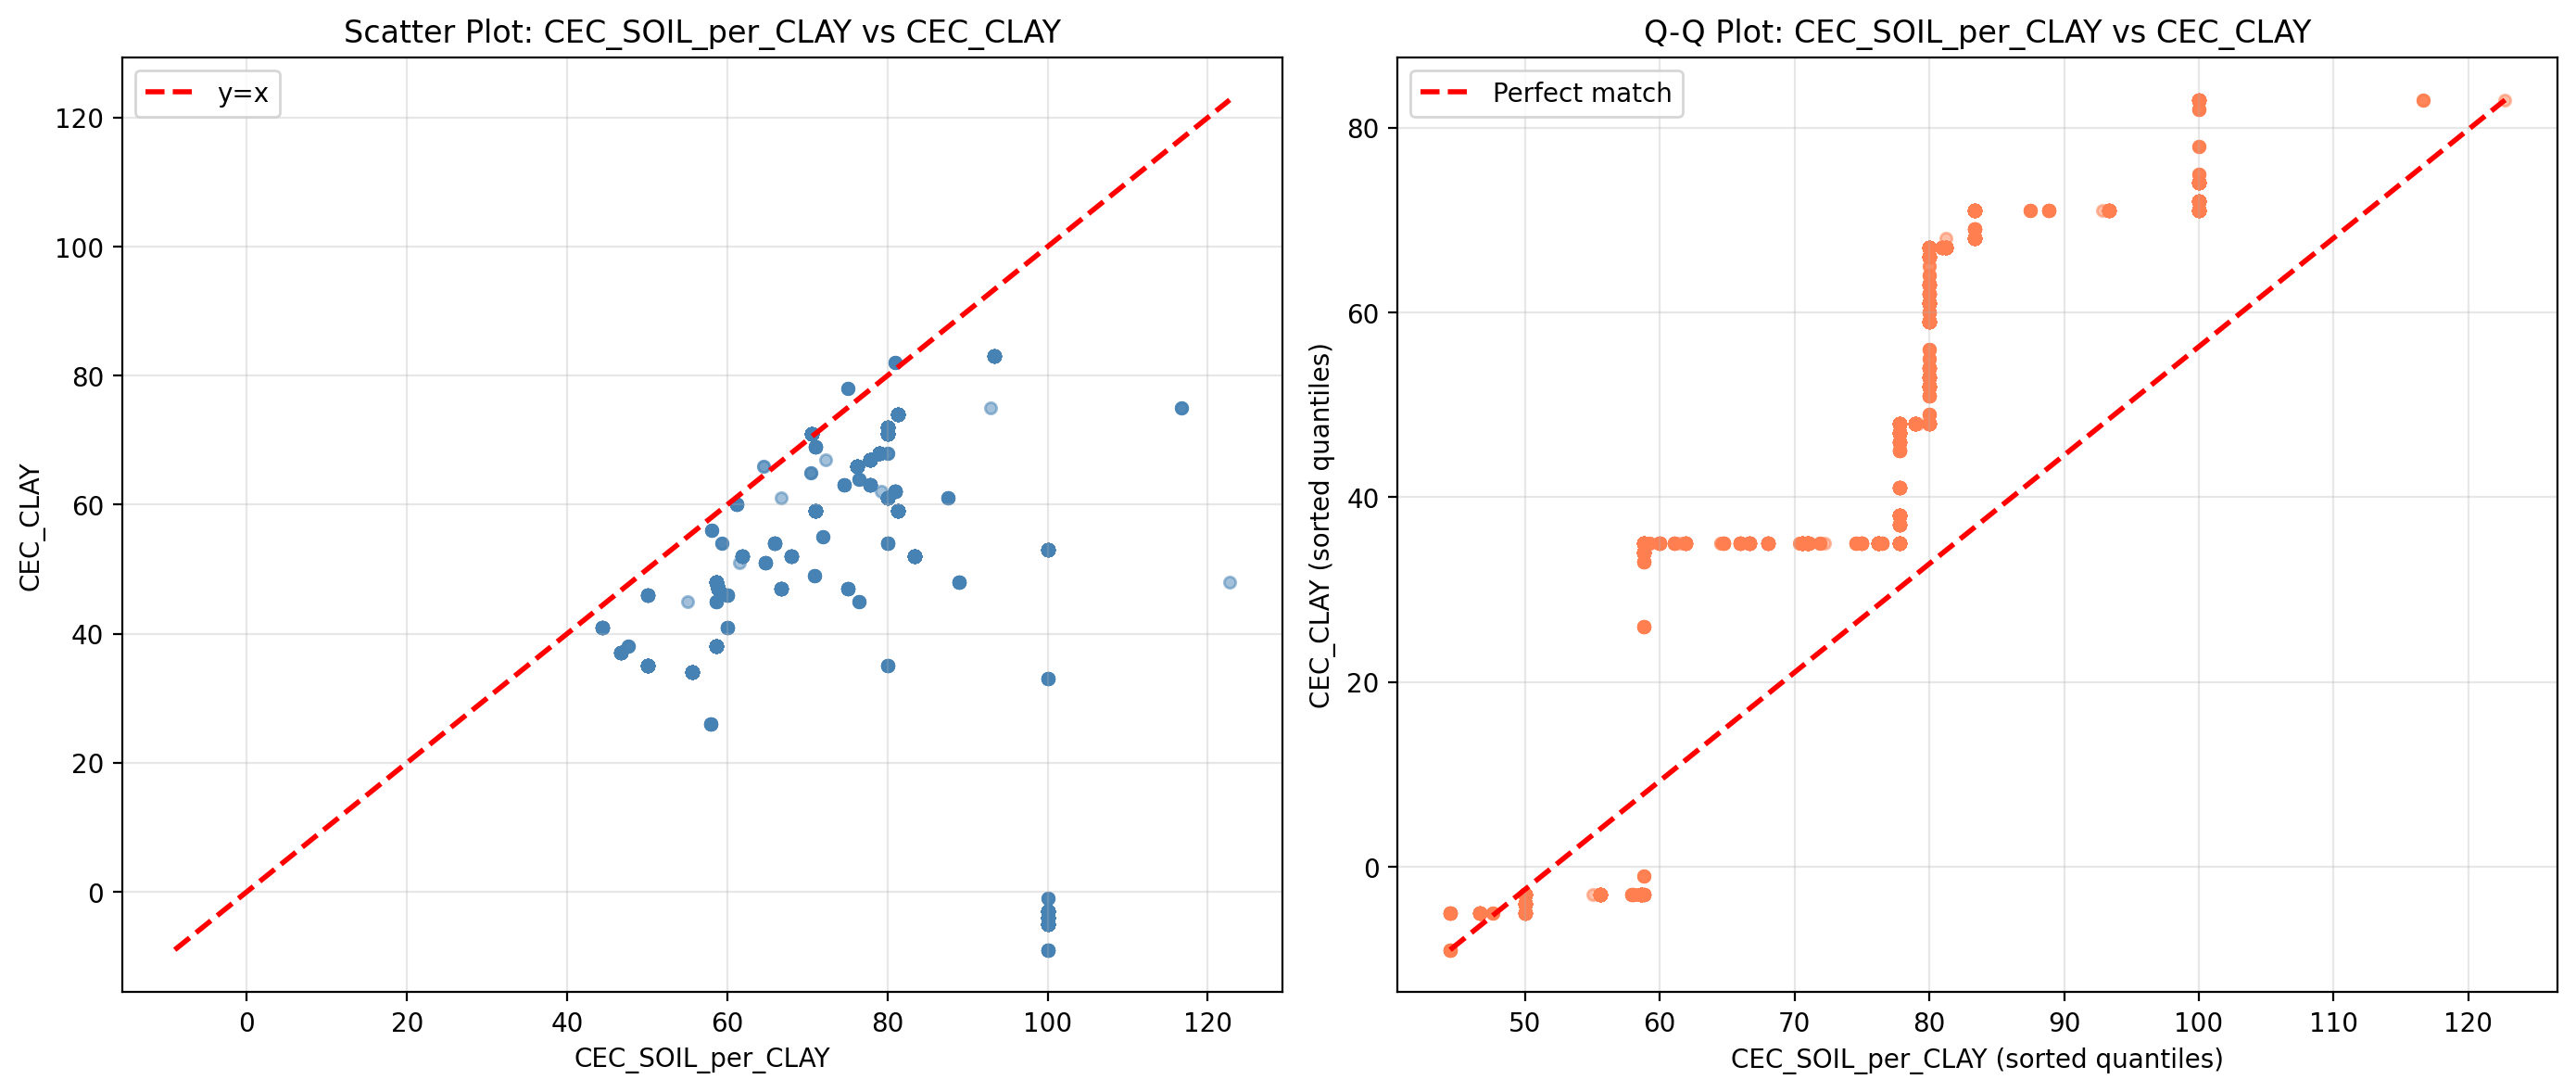
\includegraphics[width=0.55\textwidth]{images/Soil/soil_CEC_SOIL_per_CLAY_vs_CEC_CLAY_scatter_qq.png}
\caption{Scatter and Q-Q plots comparing \texttt{CEC\_SOIL\_per\_CLAY} with observed \texttt{CEC\_CLAY}, showing substantial deviation from a one-to-one relationship.}\label{fig:cec_clay}
\end{figure}

\subsubsection{Redundancy Between \texttt{TEB}, \texttt{CEC\_EFF}, and \texttt{BSAT}}

Base saturation (\texttt{BSAT}) represents the proportion of a soil's cation exchange capacity occupied by base cations and is defined as:
\[
\text{BSAT}(\%) = \frac{\text{TEB}}{\text{CEC\_EFF}} \times 100
\]
where \texttt{TEB} is the total exchangeable bases and \texttt{CEC\_EFF} is the effective cation exchange capacity\cite{ohioline_bsat}.
Comparison of \texttt{BSAT} with the computed ratio \texttt{TEB\_per\_CEC\_EFF} shows a strong association (Pearson $r = 0.82$, $p < 0.001$); however, diagnostic plots indicate that Pearson's assumptions are violated. The scatter plot reveals a clear non-linear pattern, while the Q-Q plot exhibits a pronounced S-shape, consistent with heavy-tailed distributions and the presence of influential outliers.
Given the deterministic ratio structure of \texttt{BSAT} and the observed deviations from linearity and normality, Pearson correlation was deemed inappropriate for inference. Rank-based and graphical evidence confirms that \texttt{BSAT} is primarily a monotonic but non-linear transformation of \texttt{TEB} and \texttt{CEC\_EFF}, with residual variability arising from measurement uncertainty and rounding effects, particularly near saturation values approaching 100%.
Accordingly, \texttt{BSAT} was removed from the feature set to avoid redundancy and potential multicollinearity issues during modeling, while \texttt{TEB} and \texttt{CEC\_EFF} were retained as the primary indicators of soil chemical fertility and base saturation status.

\begin{figure}[H]
\centering
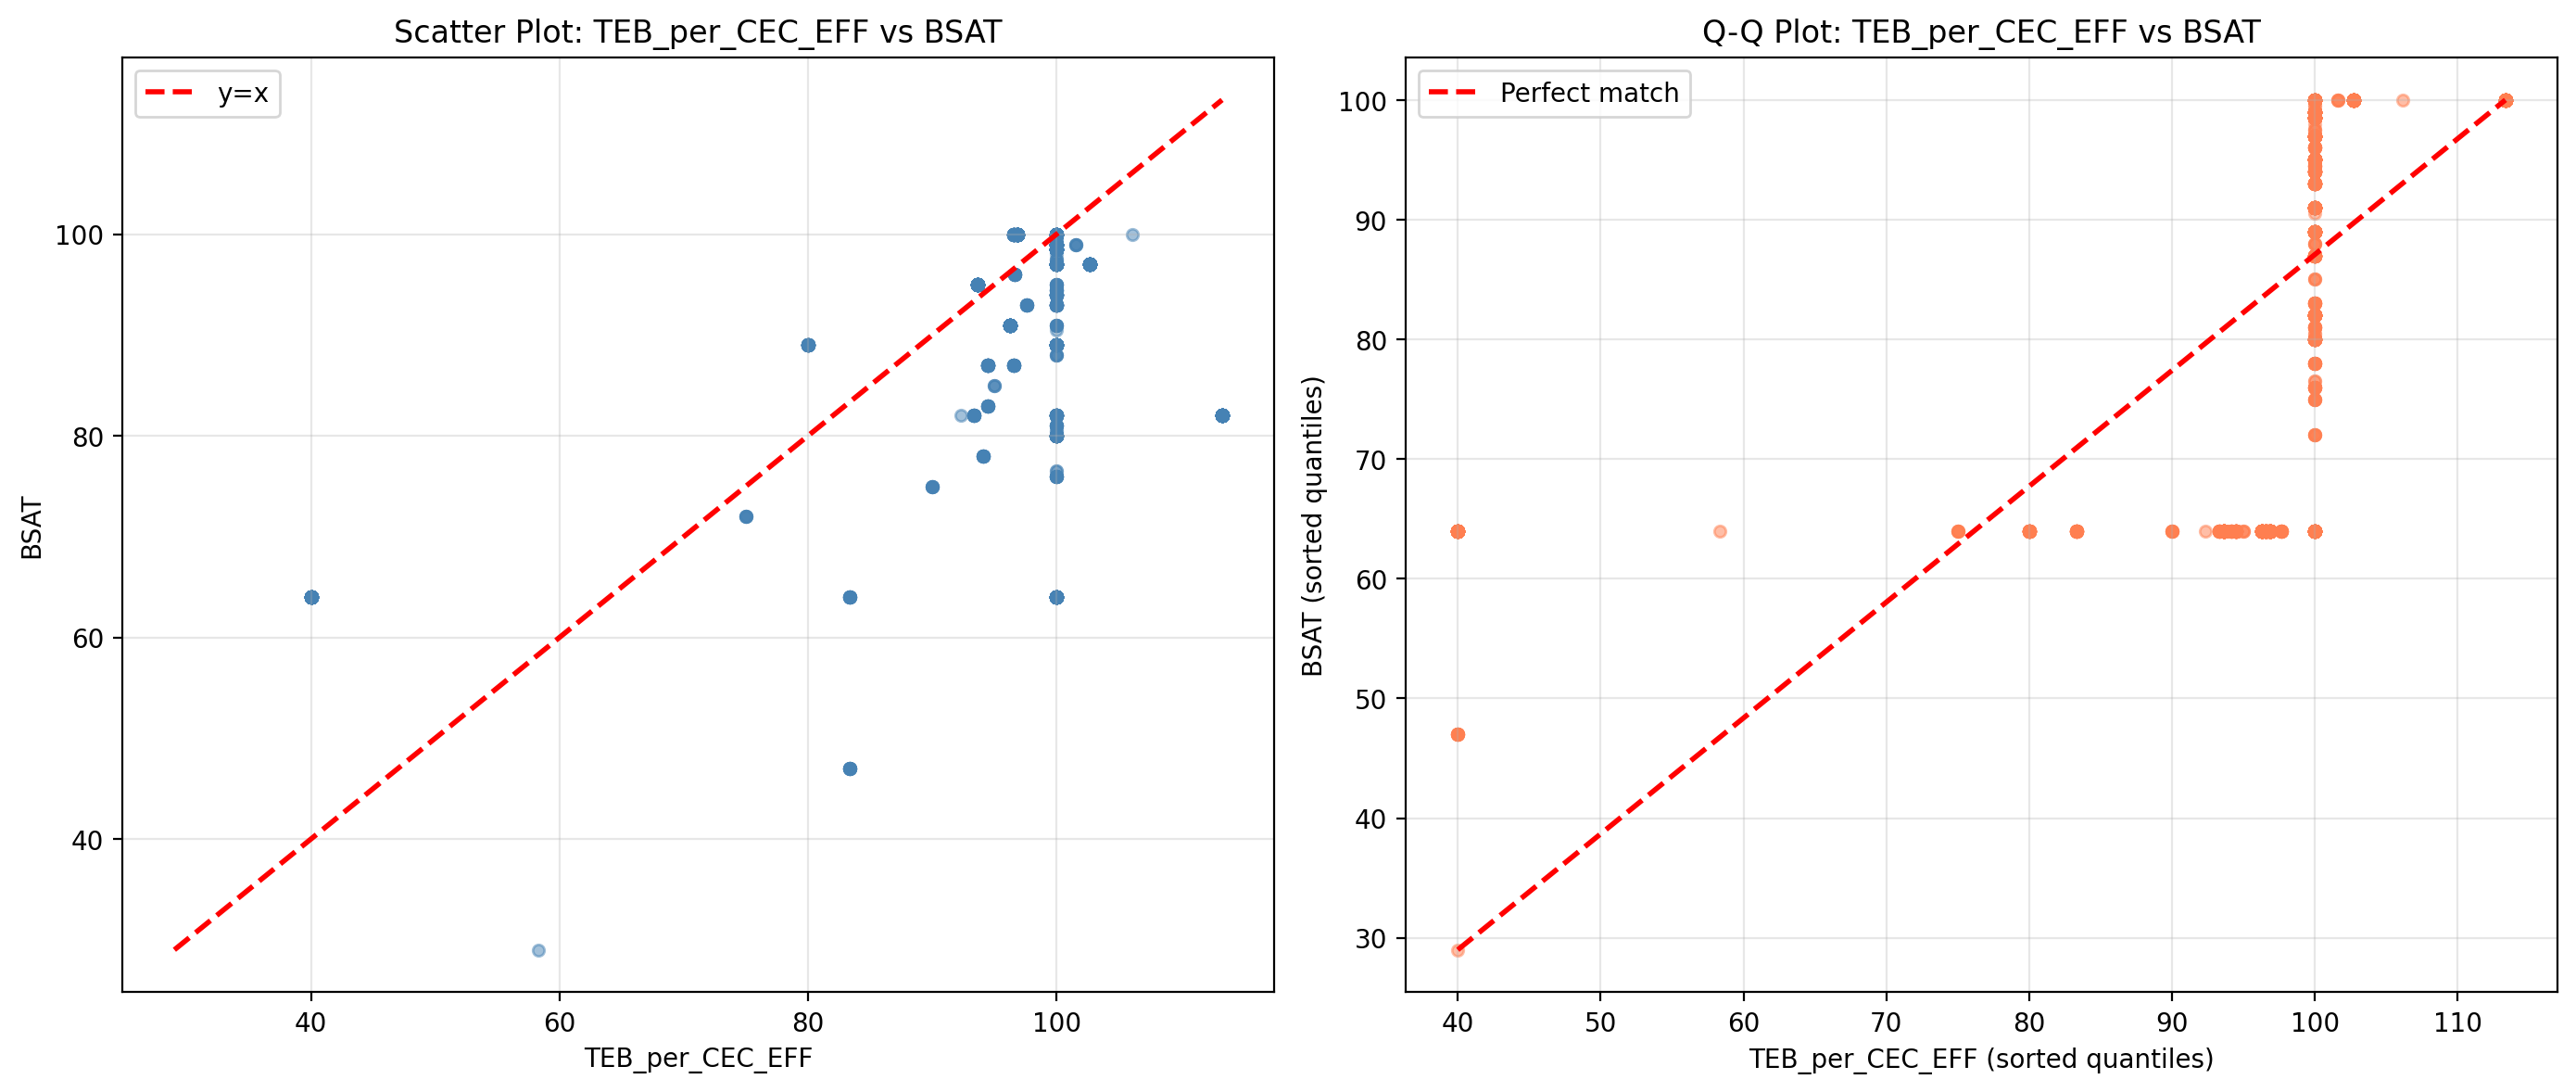
\includegraphics[width=0.55\textwidth]{images/Soil/soil_TEB_per_CEC_EFF_vs_BSAT_scatter_qq.png}
\caption{Scatter and Q-Q plots illustrating the strong dependency between \texttt{BSAT} and the computed ratio \texttt{TEB / CEC\_EFF}.}\label{fig:bsat}
\end{figure}

\subsubsection{Summary of Feature Removal Decisions}

Based on theoretical definitions and empirical validation:
\begin{itemize}
    \item \texttt{TEXTURE\_USDA} and \texttt{TEXTURE\_SOTER} were removed (derived from particle-size fractions).
    \item \texttt{CN\_RATIO} was removed (directly computed from \texttt{ORG\_CARBON} and \texttt{TOTAL\_N}).
\end{itemize}

All remaining variables were retained for subsequent normalization and modeling, ensuring minimal redundancy while preserving the physical interpretability of soil properties.

% \subsection{Initiation au \textit{Feature Engineering}: identification des variables redondantes à supprimer}\label{subsec:feature_engineering_drop}

% L'objectif de cette étape est de réduire la redondance et la multicolinéarité avant l'entraînement des modèles, en identifiant les variables qui sont des \emph{encodages déterministes} ou des \emph{indicateurs calculés} à partir d'autres colonnes déjà présentes. Cette simplification améliore la stabilité numérique, limite le risque de sur-apprentissage, et rend l'interprétation des modèles plus fiable.

% \subsubsection{Variables de texture: \texttt{TEXTURE\_USDA} et \texttt{TEXTURE\_SOTER}}\label{subsubsec:texture_drop}

% Dans le jeu de données, les modalités observées sont:
% \begin{itemize}
%   \item \texttt{TEXTURE\_SOTER}: \{M, C, -, F\}
%   \item \texttt{TEXTURE\_USDA}: \{3, 5, 9, 10, 11, 12\}
% \end{itemize}

% La Figure~\ref{fig:parallel_texture} montre des \textit{parallel coordinates} comparant \texttt{SAND}, \texttt{SILT} et \texttt{CLAY} selon \texttt{TEXTURE\_USDA} (gauche) et \texttt{TEXTURE\_SOTER} (droite). On observe des trajectoires quasi identiques au sein de chaque classe et des séparations nettes entre classes. Ceci confirme que \texttt{TEXTURE\_USDA} est un codage catégoriel dérivé directement des proportions \texttt{SAND/SILT/CLAY} (principe du triangle textural USDA), et que \texttt{TEXTURE\_SOTER} correspond également à une discrétisation des mêmes fractions granulométriques en classes (fine / medium / coarse) \cite{usda_texture, soter_texture}. Autrement dit, ces deux colonnes ne portent pas d'information indépendante supplémentaire : elles sont déterminées par \texttt{SAND}, \texttt{SILT} et \texttt{CLAY}.

% \textbf{Décision :} pour éviter la redondance et la multicolinéarité, nous supprimons :
% \[
% \boxed{\texttt{TEXTURE\_USDA},\ \texttt{TEXTURE\_SOTER}}
% \]
% tout en conservant \texttt{SAND}, \texttt{SILT}, \texttt{CLAY} (et \texttt{COARSE} si utilisé séparément).

% \begin{figure}[H]
%   \centering
%   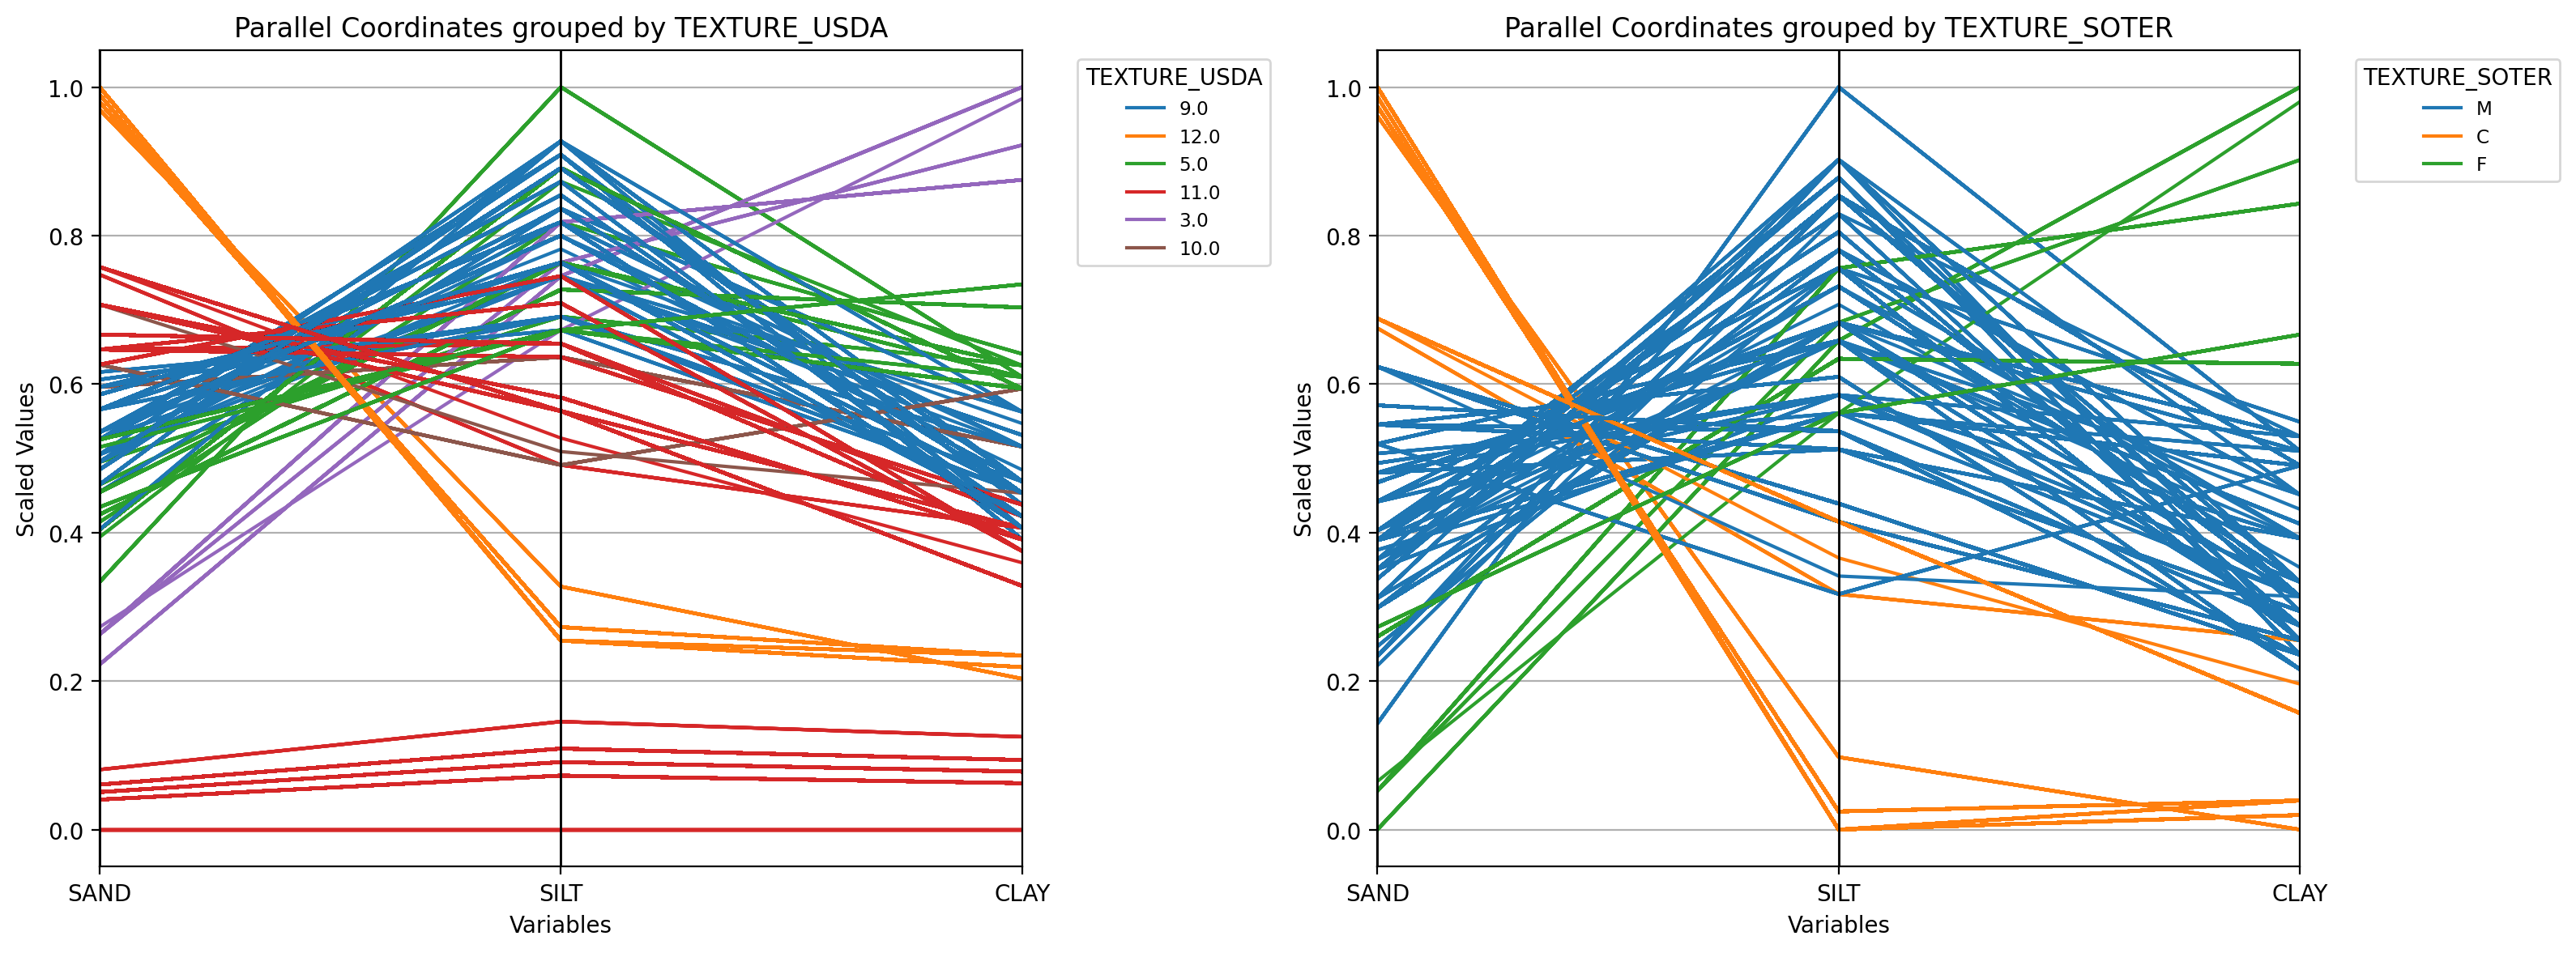
\includegraphics[width=0.98\linewidth]{images/Soil/soil_parallel_coordinates_texture.png}
%   \caption{Coordonnées parallèles des fractions granulométriques (\texttt{SAND}, \texttt{SILT}, \texttt{CLAY}) groupées par \texttt{TEXTURE\_USDA} (gauche) et \texttt{TEXTURE\_SOTER} (droite). Les classes sont des encodages dérivés des mêmes variables de base.}\label{fig:parallel_texture}
% \end{figure}

% \subsubsection{Redondance de \texttt{CN\_RATIO} avec \texttt{ORG\_CARBON} et \texttt{TOTAL\_N}}\label{subsubsec:cnratio_drop}

% Le rapport C/N (\texttt{CN\_RATIO}) est un indicateur classique de la dynamique de la matière organique. Dans la documentation HWSD2, il est défini (ou dérivé) à partir du carbone organique et de l'azote total :
% \begin{equation}
% \texttt{CN\_RATIO} = \frac{\texttt{ORG\_CARBON}}{\texttt{TOTAL\_N}}.
% \label{eq:cnratio_def}
% \end{equation}\cite{hwsd2}

% La Figure~\ref{fig:cnratio_scatterqq} (nuage de points et Q-Q) montre une relation quasi proportionnelle entre \texttt{CN\_RATIO} et la quantité recalculée \texttt{ORG\_CARBON}/\texttt{TOTAL\_N}. Cette dépendance est cohérente avec des corrélations très élevées (Pearson $r=0{,}92$, Spearman $\rho=0{,}79$, $p<0{,}001$), et les écarts résiduels s'expliquent par des effets de précision/arrondis lors de la génération des attributs.

% \textbf{Décision :} puisque \texttt{CN\_RATIO} est un indicateur calculé à partir de variables déjà disponibles, nous le supprimons:
% \[
% \boxed{\texttt{CN\_RATIO}}
% \]
% et conservons \texttt{ORG\_CARBON} et \texttt{TOTAL\_N} (plus interprétables et plus flexibles pour l'ingénierie de variables).

% \begin{figure}[H]
%   \centering
%   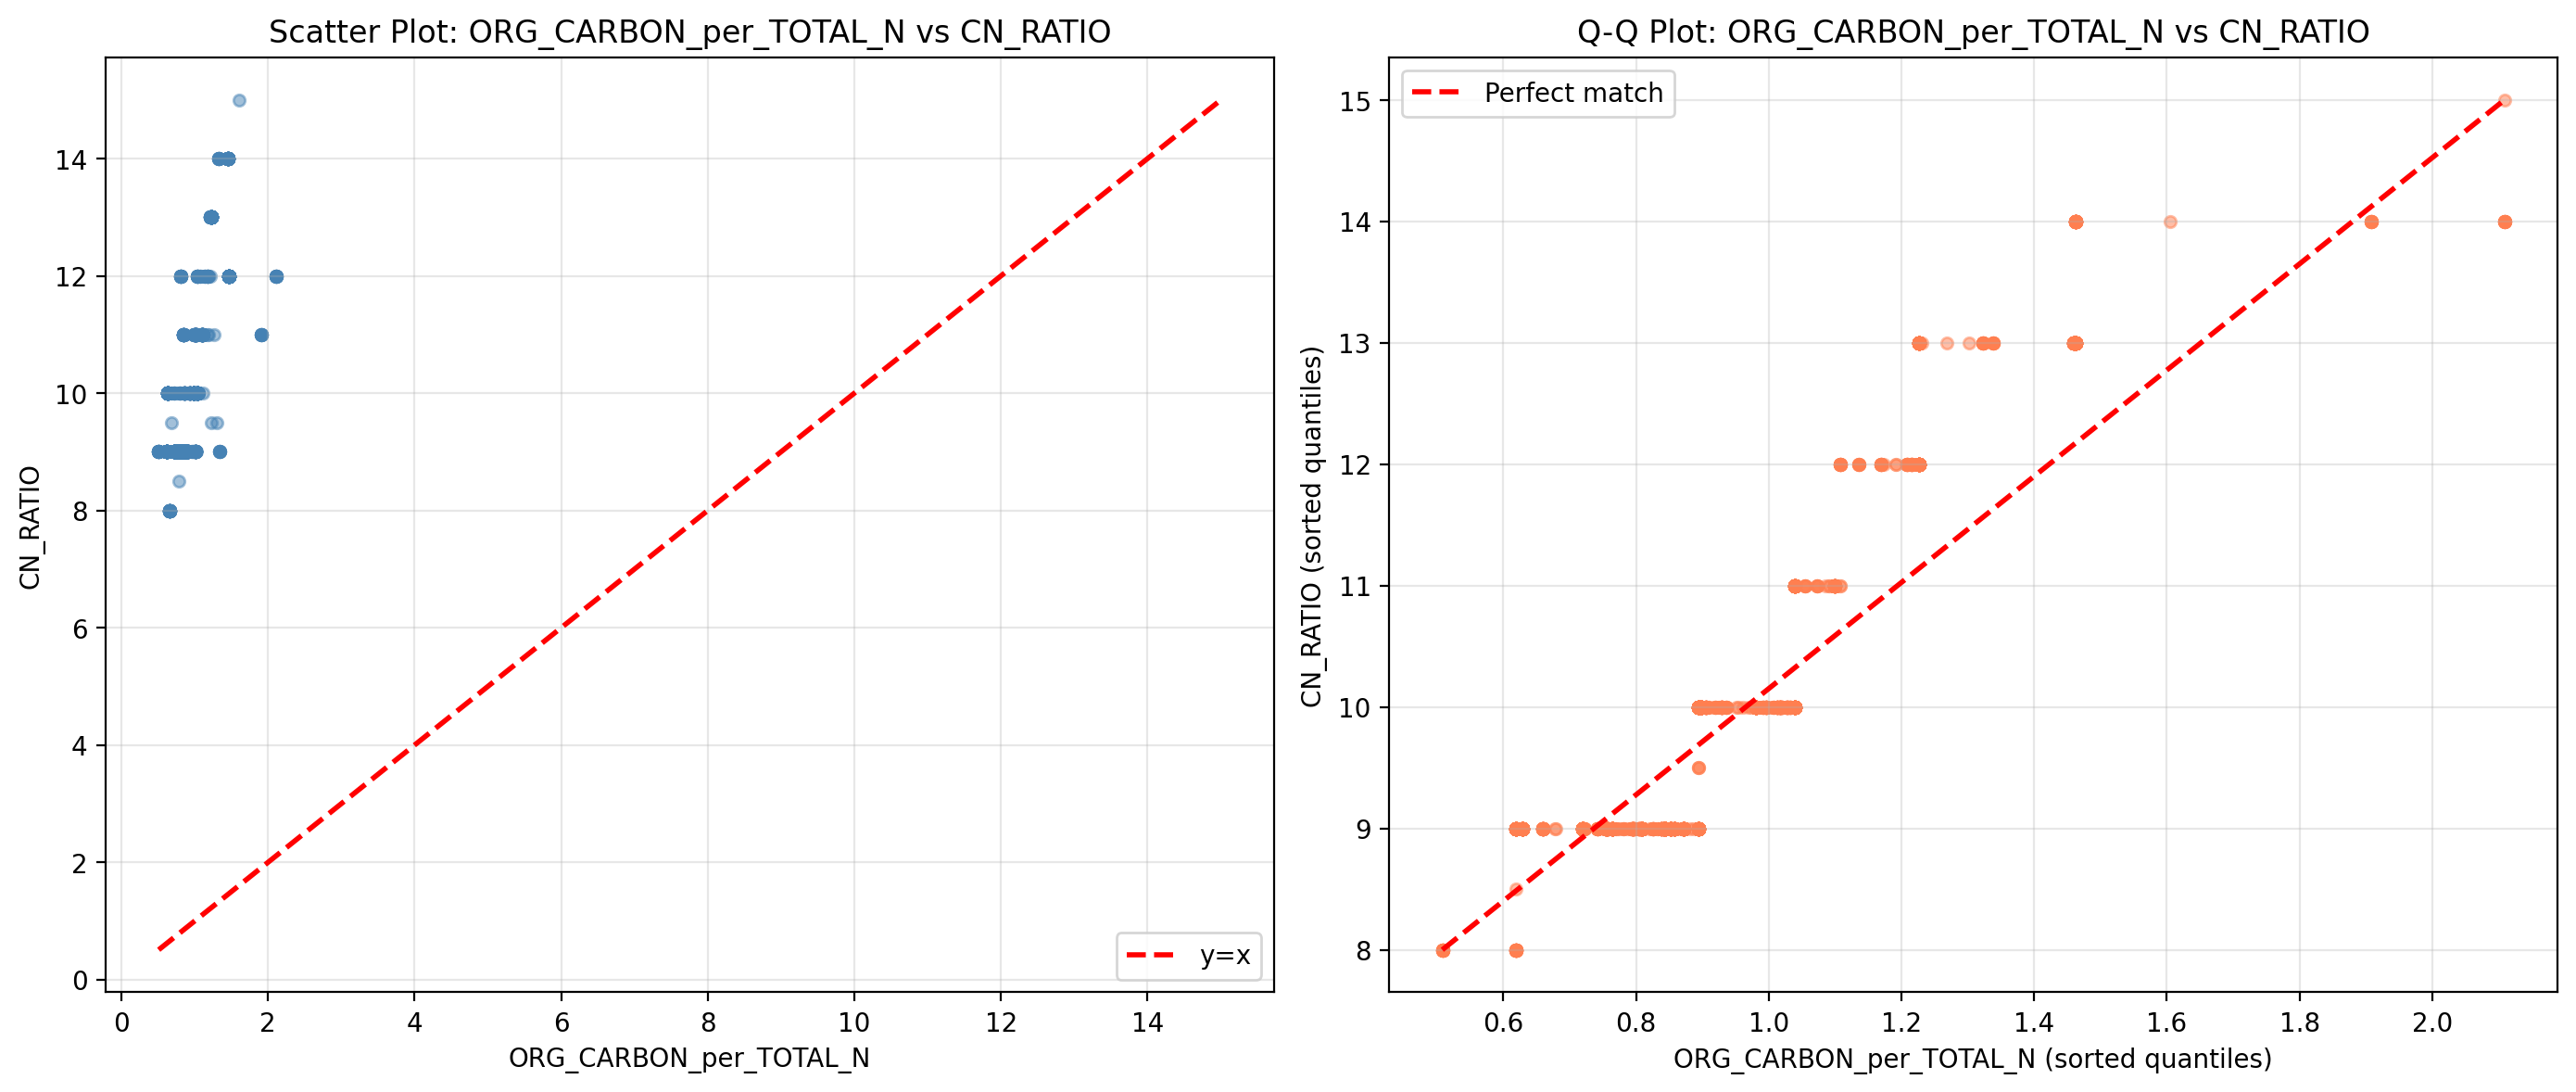
\includegraphics[width=0.98\linewidth]{images/Soil/soil_ORG_CARBON_per_TOTAL_N_vs_CN_RATIO_scatter_qq.png}
%   \caption{Vérification de la redondance de \texttt{CN\_RATIO}: comparaison entre \texttt{CN\_RATIO} et \texttt{ORG\_CARBON}/\texttt{TOTAL\_N}. L'alignement proche de $y=x$ confirme une relation dérivée.}\label{fig:cnratio_scatterqq}
% \end{figure}

% \subsubsection{Lien \texttt{CEC\_SOIL}--\texttt{CEC\_CLAY}: corrélation mais non redondance}\label{subsubsec:cec_keep}

% Théoriquement, la CEC de l'argile (\texttt{CEC\_CLAY}) est souvent présentée comme une relation entre la CEC totale du sol (\texttt{CEC\_SOIL}) et la fraction argileuse :
% \begin{equation}
% \texttt{CEC\_CLAY} \approx \frac{\texttt{CEC\_SOIL}}{\texttt{CLAY fraction}}.\label{eq:cecclay_def}
% \end{equation}\cite{hwsd2, cec_background_share}

% Cependant, la Figure~\ref{fig:cec_scatterqq} montre que le ratio calculé \texttt{CEC\_SOIL\_per\_CLAY} ne reproduit pas fidèlement \texttt{CEC\_CLAY} : dispersion marquée autour de la droite $y=x$, et déviation évidente dans le Q-Q plot. Les corrélations observées (Pearson $r=-0{,}37$, Spearman $\rho=-0{,}15$, $p<0{,}001$) confirment l'absence de dépendance déterministe. Cela est cohérent avec le fait que la CEC du sol ne dépend pas uniquement de l'argile : la matière organique, les oxydes, la minéralogie, ainsi que la fraction limoneuse peuvent contribuer significativement à la capacité d'échange.

% \textbf{Décision :} \texttt{CEC\_CLAY} n'est \emph{pas} redondante avec \texttt{CEC\_SOIL} et \texttt{CLAY}. Nous \textbf{conservons} \texttt{CEC\_CLAY}.

% \begin{figure}[H]
%   \centering
%   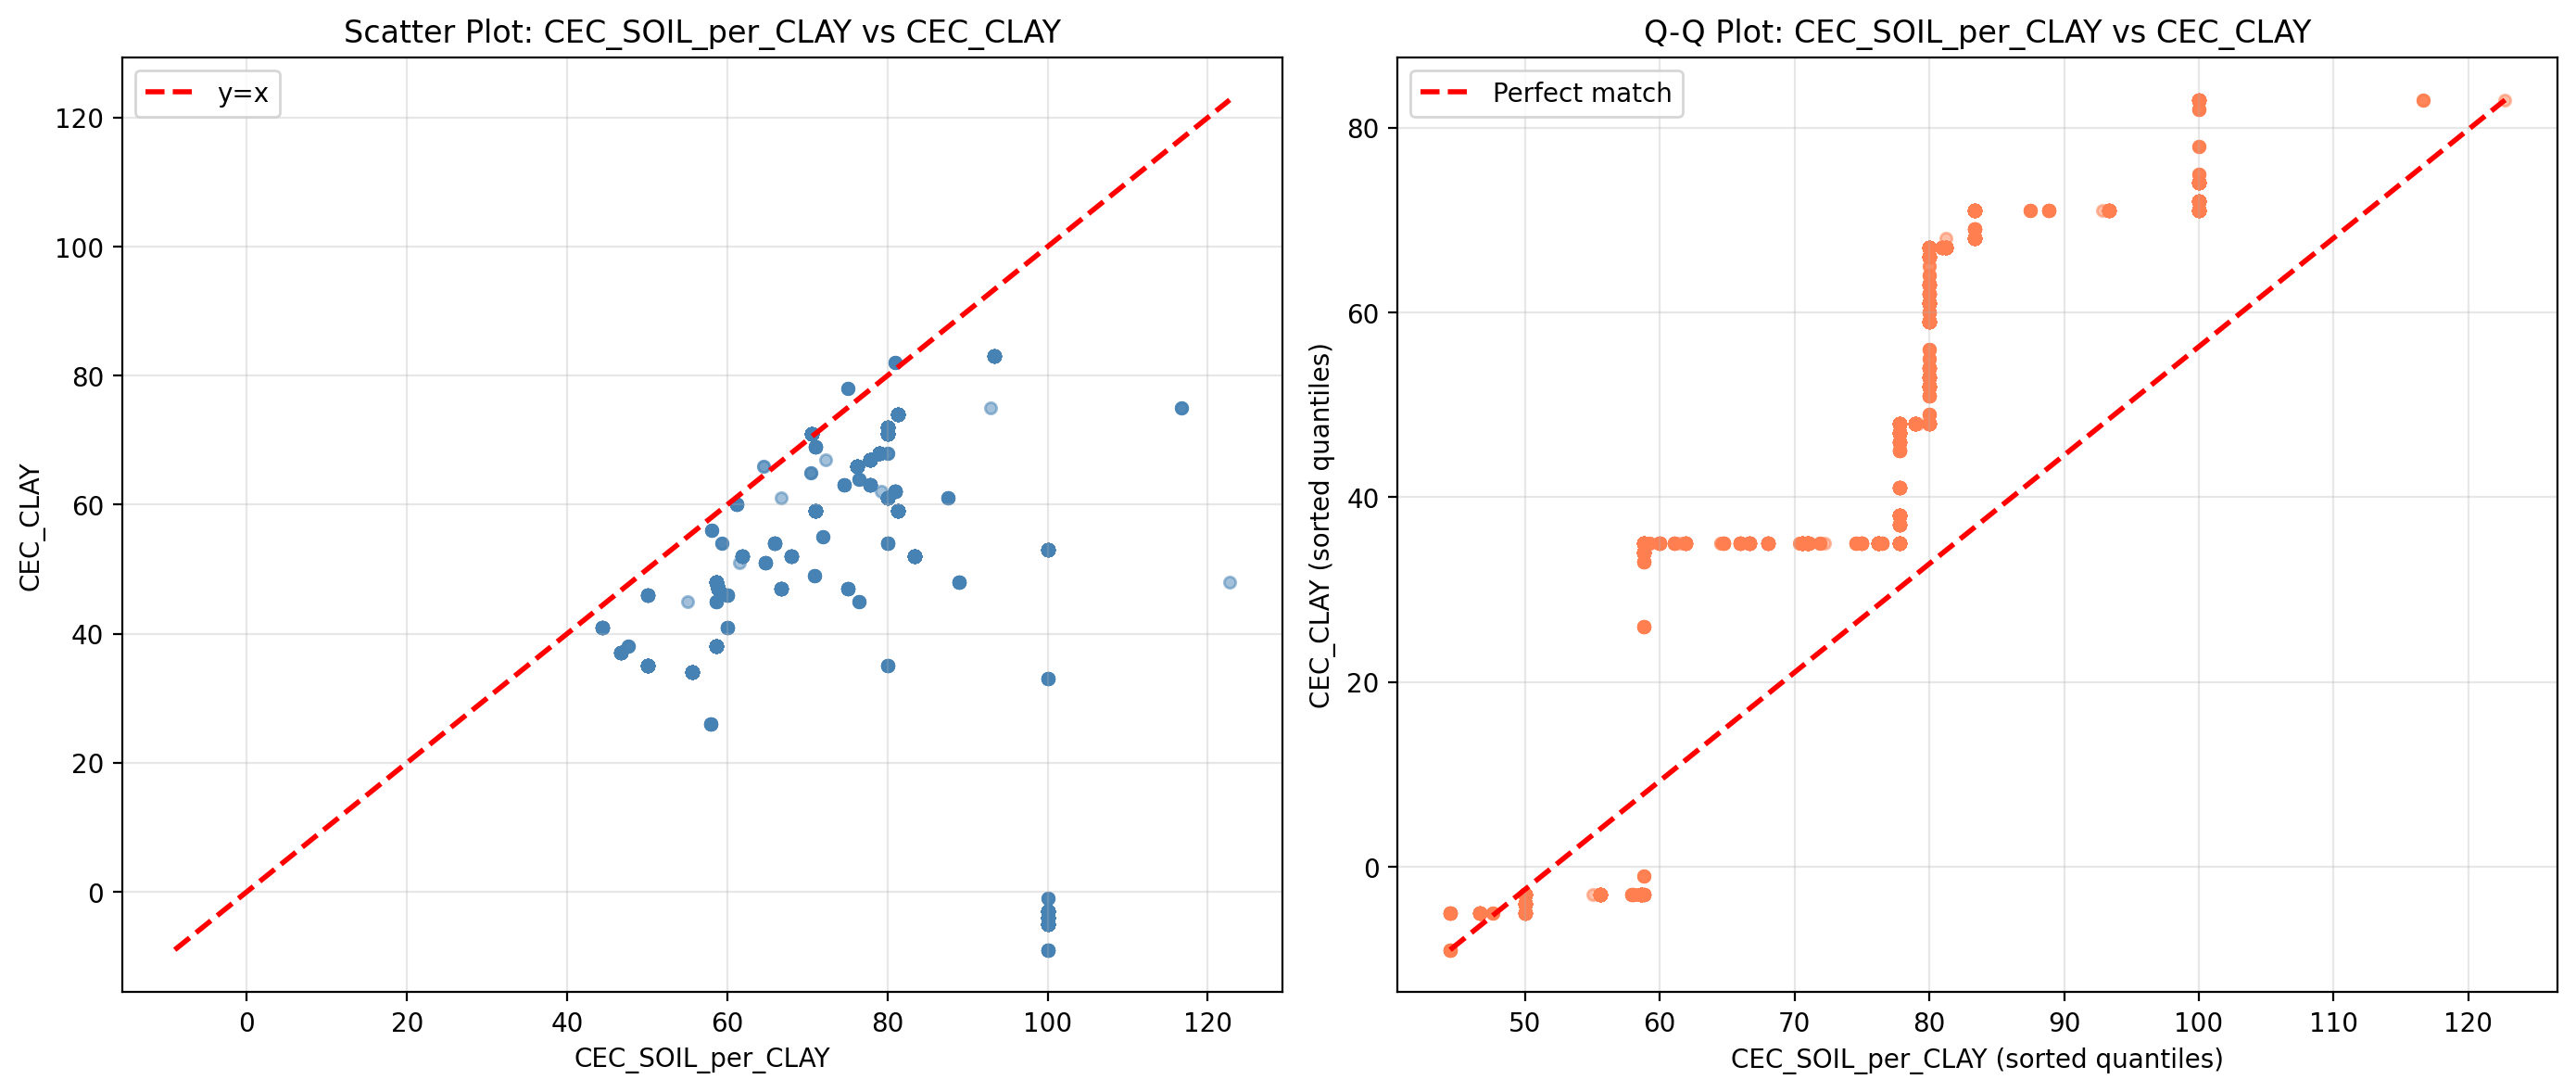
\includegraphics[width=0.98\linewidth]{images/Soil/soil_CEC_SOIL_per_CLAY_vs_CEC_CLAY_scatter_qq.png}
%   \caption{Relation entre \texttt{CEC\_SOIL\_per\_CLAY} et \texttt{CEC\_CLAY} (nuage de points + Q-Q). La dispersion et la non-coïncidence avec $y=x$ indiquent l'absence de redondance.}\label{fig:cec_scatterqq}
% \end{figure}

% \subsubsection{Redondance de \texttt{BSAT} avec \texttt{TEB} et \texttt{CEC\_EFF}}\label{subsubsec:bsat_drop}

% La saturation en bases (\texttt{BSAT}) est définie en science des sols comme:
% \begin{equation}
% \texttt{BSAT}(\%) = \frac{\texttt{TEB}}{\texttt{CEC\_EFF}} \times 100,
% \label{eq:bsat_def}
% \end{equation}
% où \texttt{TEB} est la somme des bases échangeables et \texttt{CEC\_EFF} la CEC effective\cite{ohioline_bsat}.

% La Figure~\ref{fig:bsat_scatterqq} montre une forte relation entre \texttt{BSAT} et l'indicateur calculé \texttt{TEB\_per\_CEC\_EFF}. Les résultats confirment un lien très marqué (Pearson $r=0{,}82$, $p<0{,}001$). Les déviations restantes (notamment près de \texttt{BSAT} $\approx 100\%$) sont compatibles avec des effets de plafonnement, de précision et de variabilité locale.

% \textbf{Décision :} \texttt{BSAT} étant un indicateur calculé directement à partir de \texttt{TEB} et \texttt{CEC\_EFF}, nous le supprimons :
% \[
% \boxed{\texttt{BSAT}}
% \]
% et conservons \texttt{TEB} et \texttt{CEC\_EFF}.

% \begin{figure}[H]
%   \centering
%   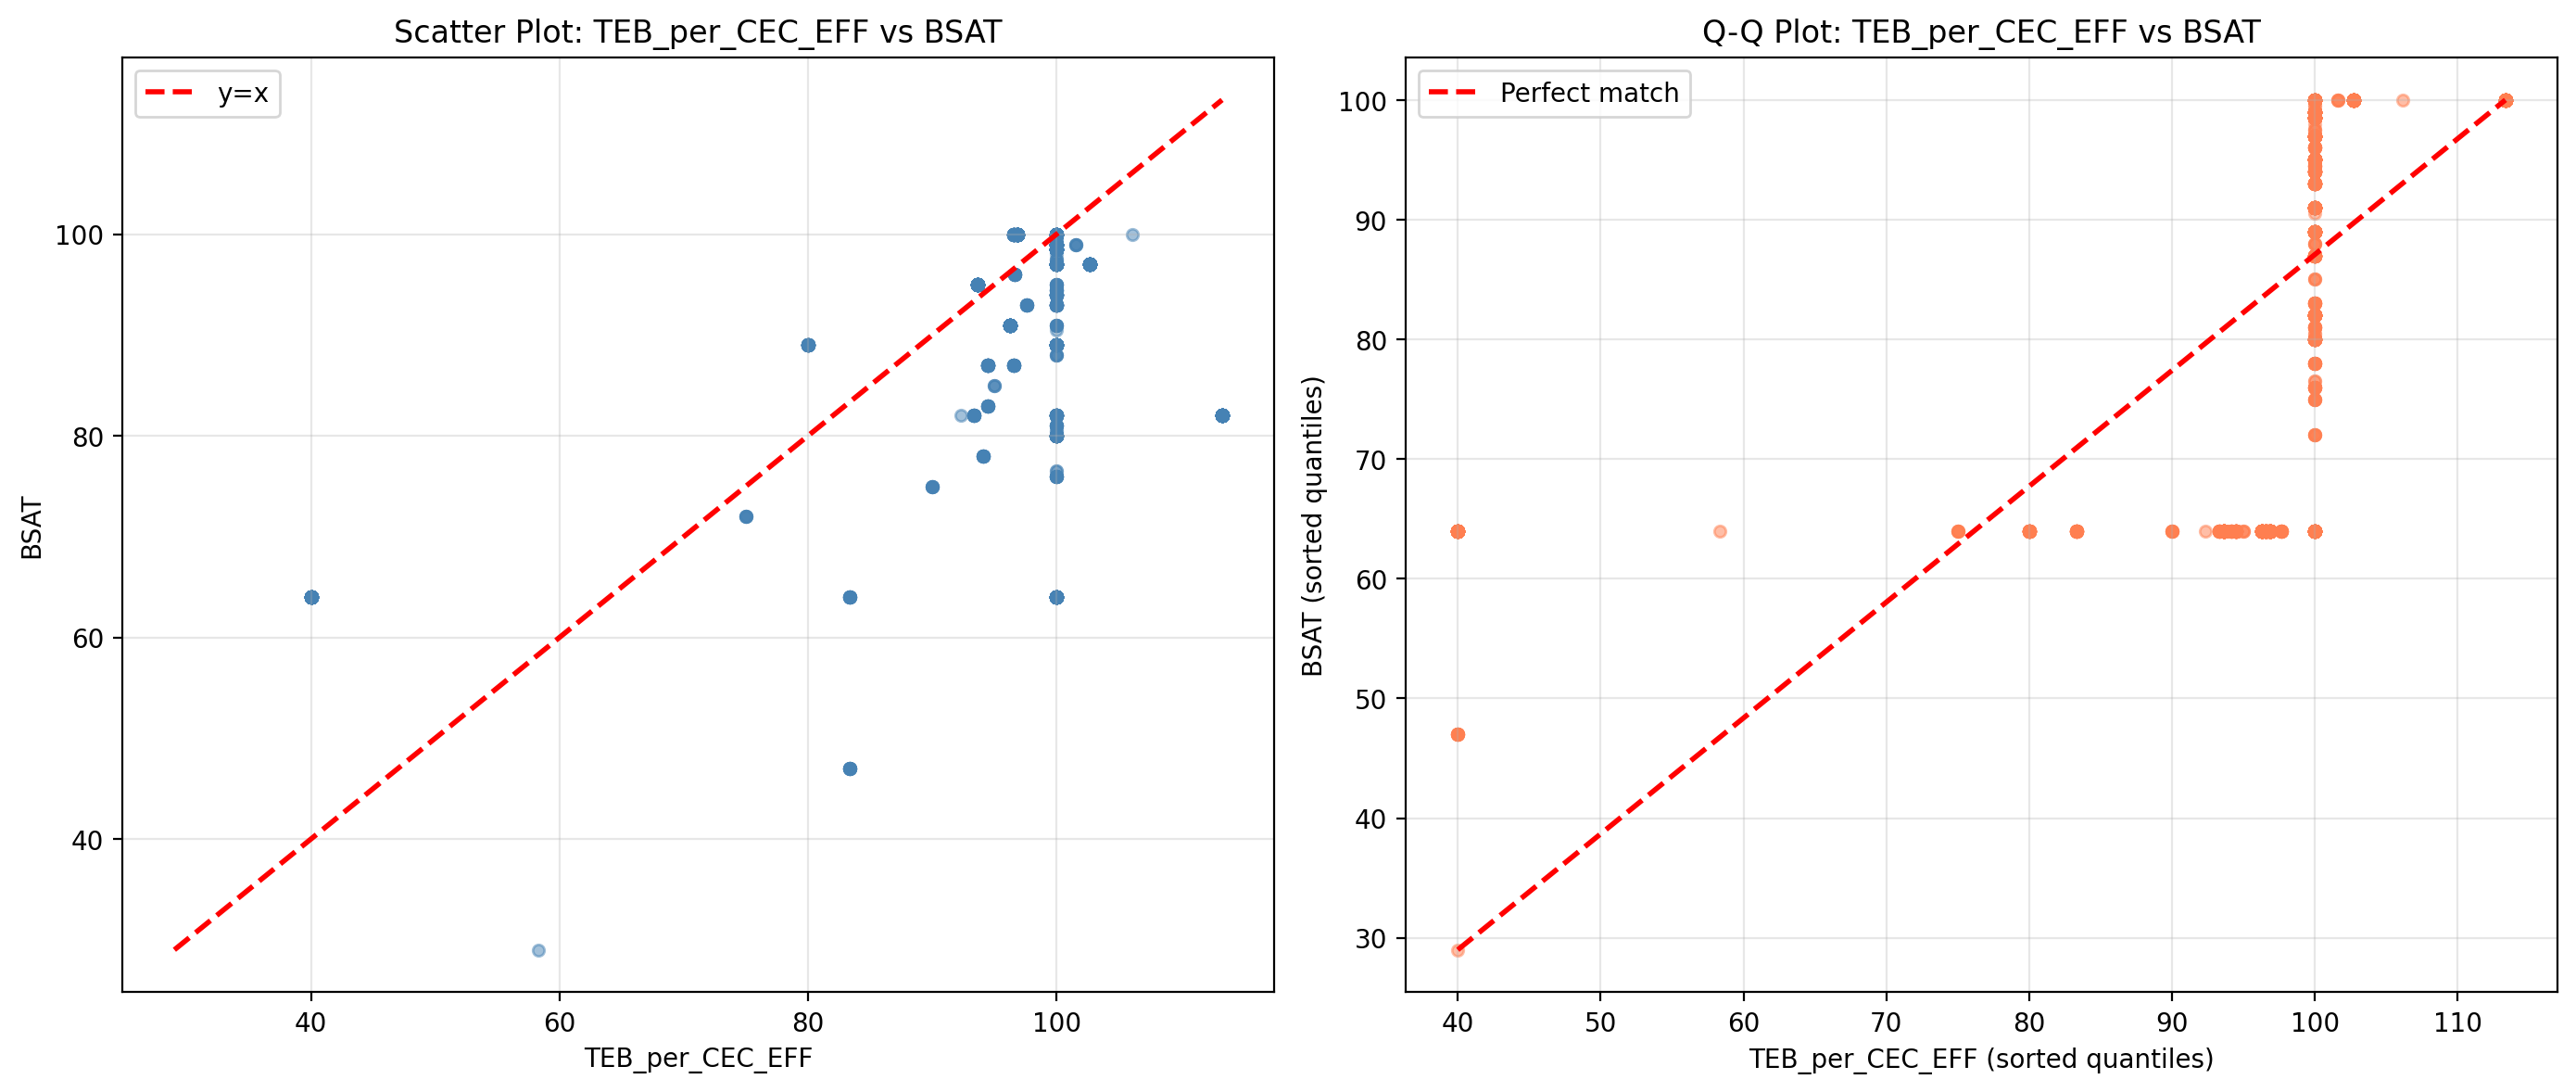
\includegraphics[width=0.98\linewidth]{images/Soil/soil_TEB_per_CEC_EFF_vs_BSAT_scatter_qq.png}
%   \caption{Vérification de la redondance de \texttt{BSAT}: comparaison entre \texttt{BSAT} et \texttt{TEB}/\texttt{CEC\_EFF} $\times 100$. L'alignement global confirme une variable dérivée.}\label{fig:bsat_scatterqq}
% \end{figure}

% \subsubsection{Synthèse: colonnes supprimées et colonnes conservées}\label{subsubsec:drop_summary}

% Au terme de cette initiation au \textit{feature engineering}, les colonnes suivantes sont considérées redondantes et supprimées :
% \[
% \boxed{\texttt{TEXTURE\_USDA},\ \texttt{TEXTURE\_SOTER},\ \texttt{CN\_RATIO},\ \texttt{BSAT}}
% \]
% Les variables de base correspondantes (\texttt{SAND}, \texttt{SILT}, \texttt{CLAY}, \texttt{ORG\_CARBON}, \texttt{TOTAL\_N}, \texttt{TEB}, \texttt{CEC\_EFF}) sont conservées, et \texttt{CEC\_CLAY} est maintenue car elle apporte une information chimique distincte (non substituable par un simple ratio).

